\chapter{Software}

\section{\textit{Product Design}}

\par O \textit{design} do produto é o processo que os \textit{designers} usam para combinar as necessidades do usuário com os objetivos de negócio para criar produtos e experiências de sucesso. 

\subsection{\textit{User Centered Design}}

\par \textit{User Centered Design} (Design centrado no usuário) é um termo usado para descrever os processos de \textit{design} os quais os usuários finais influenciam. Alguns processos utilizam técnicas voltadas para entendimento das necessidades dos usuários em pontos específicos, como levantamento de requisitos e testes de usabilidade. Outros métodos têm o usuário como um parceiro dos \textit{designers}, tendo um grande impacto no processo de \textit{design} \cite{abras2004user}.
Para o contexto da disciplina, foram utilizadas algumas técnicas do \textit{User Centered Design} citadas nos tópicos a seguir.

\subsubsection{Entrevistas}

\par Para criar um produto que satisfaça as necessidades dos seus usuários, é necessário entender suas dores e anseios. A realização de entrevistas com usuários é um dos métodos do \textit{User Centered Design} que pode ser utilizado para esse fim.
Existem quatro técnicas bastante difundidas no processo de criação de um produto: entrevistas estruturadas, semi-estruturadas, não estruturadas e por telefone. \cite{wilson2013interview}

\begin{itemize}
\item \textbf{Estruturadas} : Entrevistas com perguntas estruturadas e padronizadas, utilizadas principalmente para reunir dados demográficos, compreender o conhecimento do usuário, ou para reunir dados de atitude e de opinião.
\item \textbf{Semi-estruturadas} : O método de entrevistas semi-estruturadas utiliza uma combinação de perguntas estruturadas com a liberdade exploratória das entrevistas não estruturadas.
Ela é útil quando você tem algum conhecimento sobre um tópico, mas deseja dar aos usuários a oportunidade de levantar novas questões ou quando o tópico é muito complexo para ser uma entrevista estruturada.
\item \textbf{Não estruturadas} : Nas entrevistas não estruturadas, utilizam-se de tópicos gerais; porém, não é necessária nenhuma pergunta ou formato pré determinado. Essa entrevista é extremamente importante pra reunir dados sobre as experiências dos participantes, sem restrições. É uma conversa com um objetivo, e o rumo da entrevista pode ser ditado por ambos os participantes.
\item \textbf{Por telefone} : As entrevistas por telefone são geralmente entrevistas semiestruturadas ou estruturadas conduzidas de maneira remota.
\end{itemize}

\par Com embasamento nessas técnicas, fizemos algumas entrevistas com nossos \textit{stakeholders}. Aplicamos diferentes técnicas para cada uma das entrevistas, pois os objetivos eram diferentes.

\begin{itemize}
\item \textbf{Entrevista semi-estruturada} : A utilização da entrevista semi estruturada foi feita em um cenário complexo, onde tínhamos pouco conhecimento do assunto.
Foram criadas perguntas simples para dar objetivo inicial para a entrevista. Após isso, os próprios \textit{stakeholders} tocaram a entrevista, e os integrantes do grupo apenas complementavam com perguntas sobre o assunto. 
Essa entrevista serviu para entendermos quais dados eram gerados na simulação e quais valores eles traziam para os \textit{stakeholders}. A partir dessa entrevista, conseguimos entender quais os usos dos dados que seriam coletados e mostrados pelo nosso sistema
\item \textbf{Entrevista não estruturada} : A entrevista não estruturada foi utilizada em um contexto onde já tínhamos um conhecimento melhor sobre o assunto e queríamos validar a experiencia dos usuários com o protótipo criado.
Não foi estruturada nenhuma pergunta ou método, apenas o objetivo: validar o protótipo.
O resultado da entrevista foi uma série de apontamentos sobre a necessidade de cada usuário em cada fase de uma missão. Esses resultados foram utilizados posteriormente para criar uma evolução do protótipo.
\end{itemize}

Todas as entrevistas realizadas com os stakeholders estão disponíveis no Apêndice \ref{entrevistas} . Como as técnicas de execução das entrevistas se deram de formas variadas, algumas delas resultaram em documentos mais técnicos, outras em documentos mais informais. De toda forma, todo registro de troca de informações com o potencial usuário, é de extrema importância, pois após análise da equipe técnica podem-se derivar necessidades técnicas e demandas dos usuários que outrora não haviam sido identificadas.

\subsubsection{\textit{Brainwriting}}

\par Umas das técnicas mais populares para documentar ideias de maneira rápida é o \textit{brainstorm}. No entanto, essa técnica exige muito esforço para ser aplicada em grupo, devido à dificuldade de organização das ideias e ao gerenciamento de conflitos. O \textit{brainwriting} é a aplicação da técnica do \textit{brainstorm} de maneira silenciosa, proposto para substituir o \textit{brainstorm} em grupos. “Brainwriting é a geração silenciosa e escrita de ideias por um grupo de pessoas”. \cite{vangundy1984brain}

\par Existem 6 maneiras distintas de se fazer um \textit{brainwriting}, são elas:

\begin{itemize}
\item \textit{Nominal Group Technique} (NGT)
\item \textit{Collective Notebook} (CNB)
\item \textit{Brainwriting Pool}
\item \textit{Pin Cards}
\item \textit{Battelle-Bildmappen-Brainwriting} (BBB)
\item \textit{SIL Method}
\end{itemize}

\par Para execução do \textit{brainwriting} no nosso contexto, foram feitas algumas adaptações a partir do entendimento e da aplicação de cada uma das técnicas. Foi utilizada uma combinação das técnicas \textit{Brainwriting Pool} e  \textit{Nominal Group Technique} (NGT), resultando na seguinte definição:

\begin{itemize}
\item O organizador deve identificar um tema central da sessão, um problema;
\item Cada participante vai usar seu espaço no MIRO para fazer um \textit{brainstorm} silencioso durante 5 minutos cronometrados;
\item Após os primeiros 5 minutos, os participantes vão usar o espaço do colega do lado pra fazer suas próprias anotações por mais 5 minutos (pode-se repetir);
\item Após a segunda ou terceira interação (dependendo do organizador), cada participante volta para seu espaço e lê suas ideias para o grupo. Nessa etapa, os integrantes podem fazer perguntas e comentários para ajudar a entender melhor a ideia em questão;
\item Após todos os integrantes terem lido e entendido o que foi feito, todas as ideias serão agrupadas de acordo com sua similaridade ou proximidade;
\item Cada participante receberá 1 estrela, 3 triângulos e 5 bolas. Os elementos valem: estrela - 5 pontos, triângulo 3 pontos, bola 1 ponto;
\item Critério de desempate: o critério de desempate é a quantidade de elementos com pontuação maior. Os integrantes terão 5 minutos para distribuir seus pontos entre as ideias selecionadas na etapa anterior;
\item Ao fim da dinâmica, é feita a contagem dos pontos e a eleição das ideias que serão aproveitadas pelo grupo, em ordem de prioridade.
\end{itemize}

\par Utilizando essa metodologia, conseguimos estabelecer uma visão compartilhada junto à equipe e aos demais envolvidos sobre o produto que seria desenvolvido. O artefato gerado, Figura \ref{fig:miro}, ajuda tanto a manter o foco e a clareza dos objetivos do produto quanto a proporcionar a horizontalidade e a distribuição de conhecimentos em relação a esse produto. O mesmo pode ainda ser acessado \href{https://miro.com/app/board/o9J_kmVCAxA=/}{aqui}.

\begin{figure}[H]
\centering
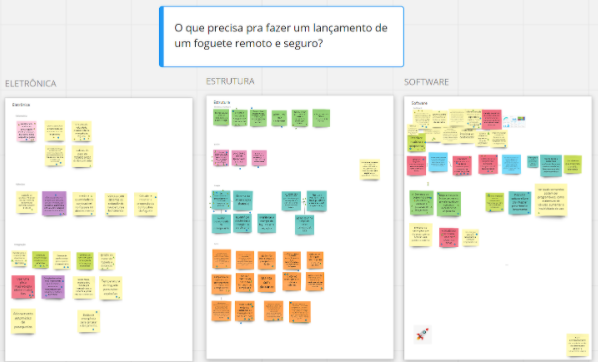
\includegraphics[scale=0.8]{figuras/miro.png}  
\caption{Brainwriting.}
\label{fig:miro}
\end{figure}

%\footnotesize Pode-se acessar em: \url{https://miro.com/app/board/o9J_kmVCAxA=/}

\subsubsection{\textit{Storyboard}}

\par Sob a perspectiva de modelos de desenvolvimento, já é comum o uso de histórias de usuários como um aspecto fundamental quando se trata de adotar o modelo \textit{eXtreme Programming}. A ideia consiste em fornecer uma visão de alto nível dos requisitos de um sistema, usadas como principal entrada de informações sobre estimativas e cronogramas, além de guiar a identificação de tarefas de desenvolvimento e conjunto de testes de aceitação (AMBLER, 2004). 

\par O \textit{storytelling} geralmente concentra-se em três linhas de pesquisas distintas: Geração, Interação ou Visualização das histórias \cite{pozzer}. Assim, nesta etapa do trabalho, a ênfase será na linha de construção que remete a forma como a história é gerada, ou seja, como se dá a elaboração da estrutura que irá guiar aspectos mais gerais, como personagens, ações, objetos e relacionamentos entre usuário e desenvolvedor para que essas especificações sejam geradas.

\par \textit{Storytelling} é um novo paradigma de entretenimento digital que está avançando a passos largos, com a criação de técnicas e ferramentas que permitem que histórias interativas possam ser criadas, visualizadas e guiadas com o auxílio do computador \cite{pozzer}.
Por fim, a “Exibição” trata a forma de representação gráfica da história, ou seja, a transformação das abstrações das estruturas internas dos personagens em ações realistas dentro de um espaço gráfico.

\par Contudo, \textit{storytelling} é mais do que um método baseado no ato de contar uma história. Tem como finalidade a captura e a transmissão de conhecimento de forma estruturada. A metodologia adotada pela equipe entrelaça conceitos de RUP e ágil, o que faz que o dinamismo e a relação com o \textit{stakeholder} sejam de fácil acesso e de muita troca de informações, tornando os requisitos mutáveis e adaptáveis à medida que o processo acontece.

\par Com base nesse contexto, o \textit{storytelling} tem como objetivo assegurar a construção das histórias de usuário com o intuito de prevenir e corrigir as falhas de comunicação e conceito de escopo que possam existir durante o processo.

\par O artefato que foi gerado pela equipe pode ser conferido nas Figuras \ref{fig:storytelling01} e \ref{fig:storytelling02}:

"\textit{Guto é um integrante de uma equipe de competição universitária de lançamento de foguetes de pequeno porte e comumente enfrenta problemas com o lançamento dos foguetes da equipe por conta da necessidade da execução manual  obrigatória de rotinas de lançamento.}
    
\textit{Além disso, as informações a respeito do lançamento e do desempenho do foguete são turvas e só podem ser obtidas após a recuperação do foguete, que acontece depois da competição.}

\begin{figure}[H]
\centering
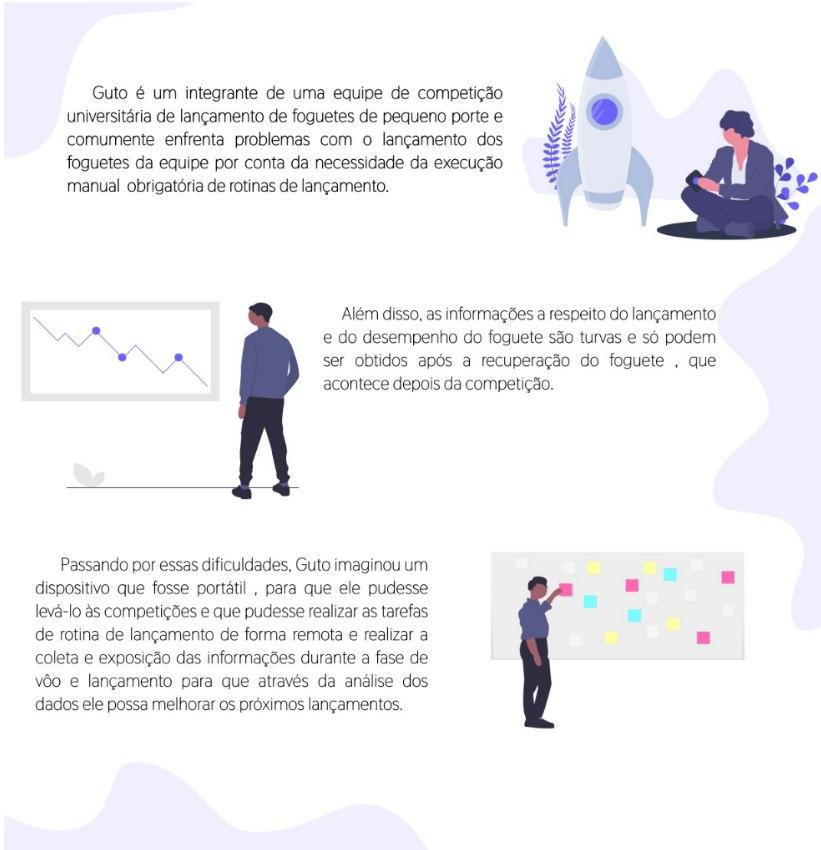
\includegraphics[width=0.8\textwidth]{figuras/storytelling1.jpg}
\caption{Storytelling: Página 1}
\label{fig:storytelling01}
\end{figure}

\textit{Passando por essas dificuldades, Guto imaginou um dispositivo que fosse portátil, para que ele pudesse levá-lo às competições, e que pudesse realizar as tarefas de rotina de lançamento de forma remota e realizar a coleta e exposição das informações durante a fase de vôo e lançamento para que através da análise dos dados ele possa melhorar os próximos lançamentos.}

\textit{Assim surgiu o  GCS , um dispositivo portátil, que, além de sanar as dificuldades de Guto, é portátil, seguro, e projetado por meio do método “user centered design”, para que as suas funcionalidades sejam intuitivas e de fácil usabilidade para o usuário.}

\begin{figure}[H]
\centering
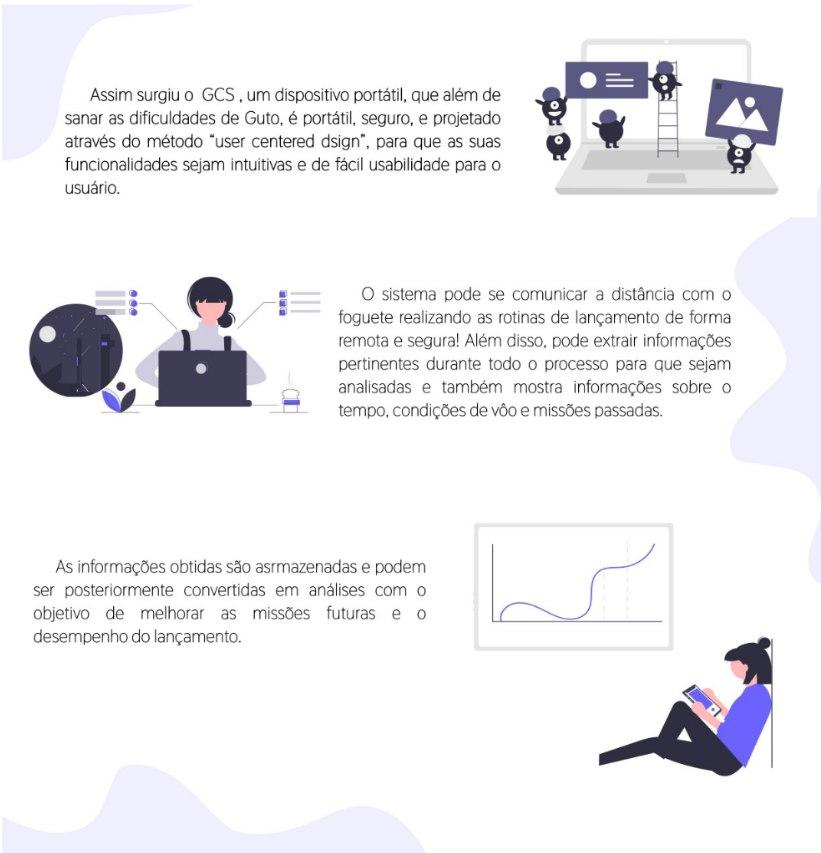
\includegraphics[width=0.9\textwidth]{figuras/sotytelling2.jpg}
\caption{Storytelling: Página 2}
\label{fig:storytelling02}
\end{figure}

\textit{O sistema pode-se comunicar à distância, com o foguete realizando as rotinas de lançamento de forma remota e segura! Além disso, pode extrair informações pertinentes durante todo o processo para que sejam analisadas e também mostra informações sobre o tempo, condições de voo e missões passadas.}"

\subsection{Arquitetura da informação}

\par A arquitetura da informação é a ciência de organizar e categorizar \textit{web sites}, intranets, comunidades \textit{online} e \textit{softwares}, para favorecer a usabilidade e a facilidade, para se encontrar o que se procura. Ou seja, é a estruturação de toda a informação disponível em um site ou aplicação, para que os usuários possam encontrar fácil e rapidamente o que procuram. E o arquiteto de informação é, na essência, o responsável por isso \cite{de2011fundamentos}. 

\par Durante a execução desta etapa do projeto, a equipe dedicou-se a executar atividades que fossem relacionadas aos princípios do \textit{User Centered Design}, e, com base nisso, à elaboração de artefatos que ajudassem a construir uma interface intuitiva para o usuário. Os artefatos elaborados pela equipe podem ser conferidos nas sessões seguintes.

\subsubsection{\textit{Wireframe}}

\par Os \textit{wireframes} são diagramas de baixa fidelidade que representam o layout de um site ou aplicação. A sua relevância no processo de \textit{design} deve‐se ao fato de permitirem explorar, testar e iterar ideias de \textit{design} numa fase inicial do projeto, momento em que as mudanças não vão aumentar o orçamento do trabalho. É importante que as pessoas responsáveis pela criação de conteúdo estejam envolvidas no processo de \textit{wireframing} \cite{brito2016usabilidade}. 

\begin{figure}[H]
\centering
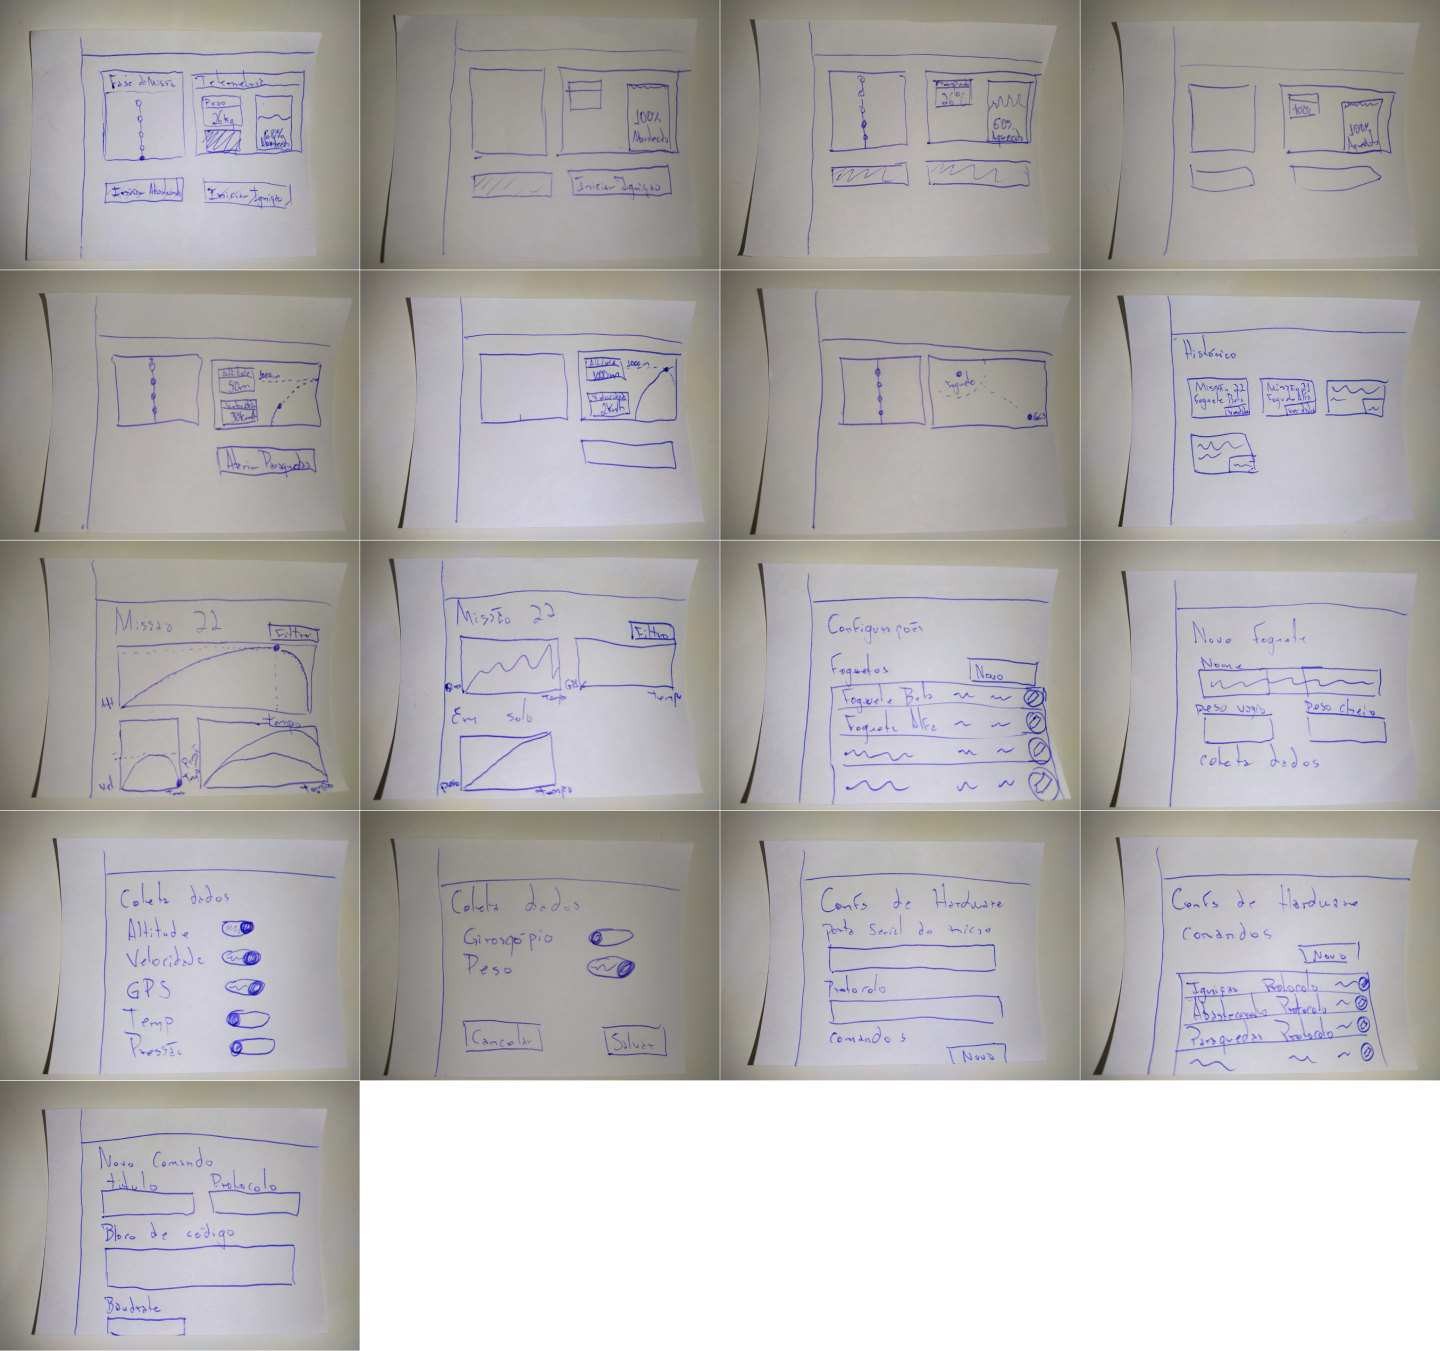
\includegraphics[scale=0.21]{figuras/wireframe.png}  
\caption{Wireframe}
\label{fig:Wireframe}
\end{figure}

\par Com o objetivo de testar as possíveis versões da interface e iterar a organização estrutural da informação da aplicação, a equipe elaborou um \textit{wireframe}, que foi validado com os usuários e \textit{stakeholders}. Esse artefato é apresentado na Figura \ref{fig:Wireframe} e também pode ser visualizado \href{https://bit.ly/3jnLnmN}{aqui}.


\subsubsection{Protótipo de média fidelidade}
\label{prototipo}

\par A prototipação no desenvolvimento de \textit{software} é um processo que tem como função avaliar as ideias geradas e validar – ou não – todos os requisitos estabelecidos \cite{lilley2004development}. É nesse momento que a equipe tende a  tirar as ideias do papel e passar a entendê-las na forma física.

\par Essa etapa é importante para verificar se a solução desenhada está adequada ao desafio que o cliente enfrenta, garantindo o alinhamento das informações. Dessa forma, consegue-se minimizar os riscos, permitindo que o cliente valide e faça todos os testes antes da implantação. É importante ressaltar que a fase de prototipação pode – e muitas vezes deve – ser realizada em diversos momentos, já que se verificam falhas de forma ágil, chegando assim a uma solução de software mais assertiva.

\par Apesar de já serem definidos diversos requisitos antes do desenvolvimento do \textit{software}, é durante a interação real do usuário com o sistema que os novos detalhes são percebidos. Para isso, a equipe realizou a elaboração de protótipos de baixa e média fidelidade, com a colaboração dos usuários e \textit{stakeholders}. As versões dos protótipos podem ser conferidas a seguir:


\href{https://bit.ly/35xe23N}{Protótipo V0}.

\href{https://bit.ly/2FW3oep}{Protótipo V1}.

\href{https://bit.ly/34pAfS2}{Protótipo V2}.

\subsection{Definição do produto}

\par O projeto aplica-se a um contexto de competições de lançamento de foguetes experimentais, onde cada equipe constrói seu foguete com base no regulamento da competição. Os projetos necessitam estar adequados o melhor possível às regras para obter uma boa pontuação. Devido à dinamicidade dos projetos e da baixa restrição de \textit{hardware} das competições, temos diversas configurações de \textit{hardware}. Nesse contexto, os sistemas de \textit{software} têm uma grande necessidade de adequação e adaptação aos diferentes \textit{hardwares} possíveis.

\par O produto de \textit{software} visa auxiliar o controle e monitoramento do lançamento de um foguete experimental para competições, provendo segurança, controle e visão de uma missão \footnote{Uma missão é todo o processo de lançamento de um foguete em uma competição. Vai desde a preparação para o abastecimento até a coleta do foguete após pousar.}. O sistema irá atuar em 3 momentos na competição:

\begin{itemize}
    \item abastecimento e ignição do foguete;
    \item foguete em voo;
    \item foguete em pouso.
\end{itemize}

\par Em ambos os momentos da competição, o sistema comunicar-se-á com \textit{hardwares} externos para fazer as leituras e enviar comandos de controles. Para tornar o produto de software valioso para os clientes, é fundamental satisfazer os objetivos e restrições expostos. Assim, faz-se necessária a construção de um sistema que permita a visualização e controle dos processos da missão, a partir de dados de telemetria e comandos para o \textit{hardware}, sendo estes configuráveis.Portanto, podemos definir as principais funcionalidades do sistema como:

\begin{itemize}
    \item Possibilitar a leitura e exposição dos dados de telemetria do foguete:
    \begin{itemize}
        \item GPS;
        \item Altitude;
        \item Velocidade;
        \item Temperatura;
        \item Pressão;
        \item Giroscópio;
        \item Peso (em solo); 
    \end{itemize}
    \item Possibilitar comandos de ignição, abastecimento e abertura do paraquedas;
    \item Possibilitar configuração dos comandos e protocolos necessários para se comunicar com diferentes \textit{hardwares};
    \item Armazenar os dados de maneira segura.
\end{itemize}

\subsubsection{Mapa de requisitos}

\begin{figure}[h!]
\centering
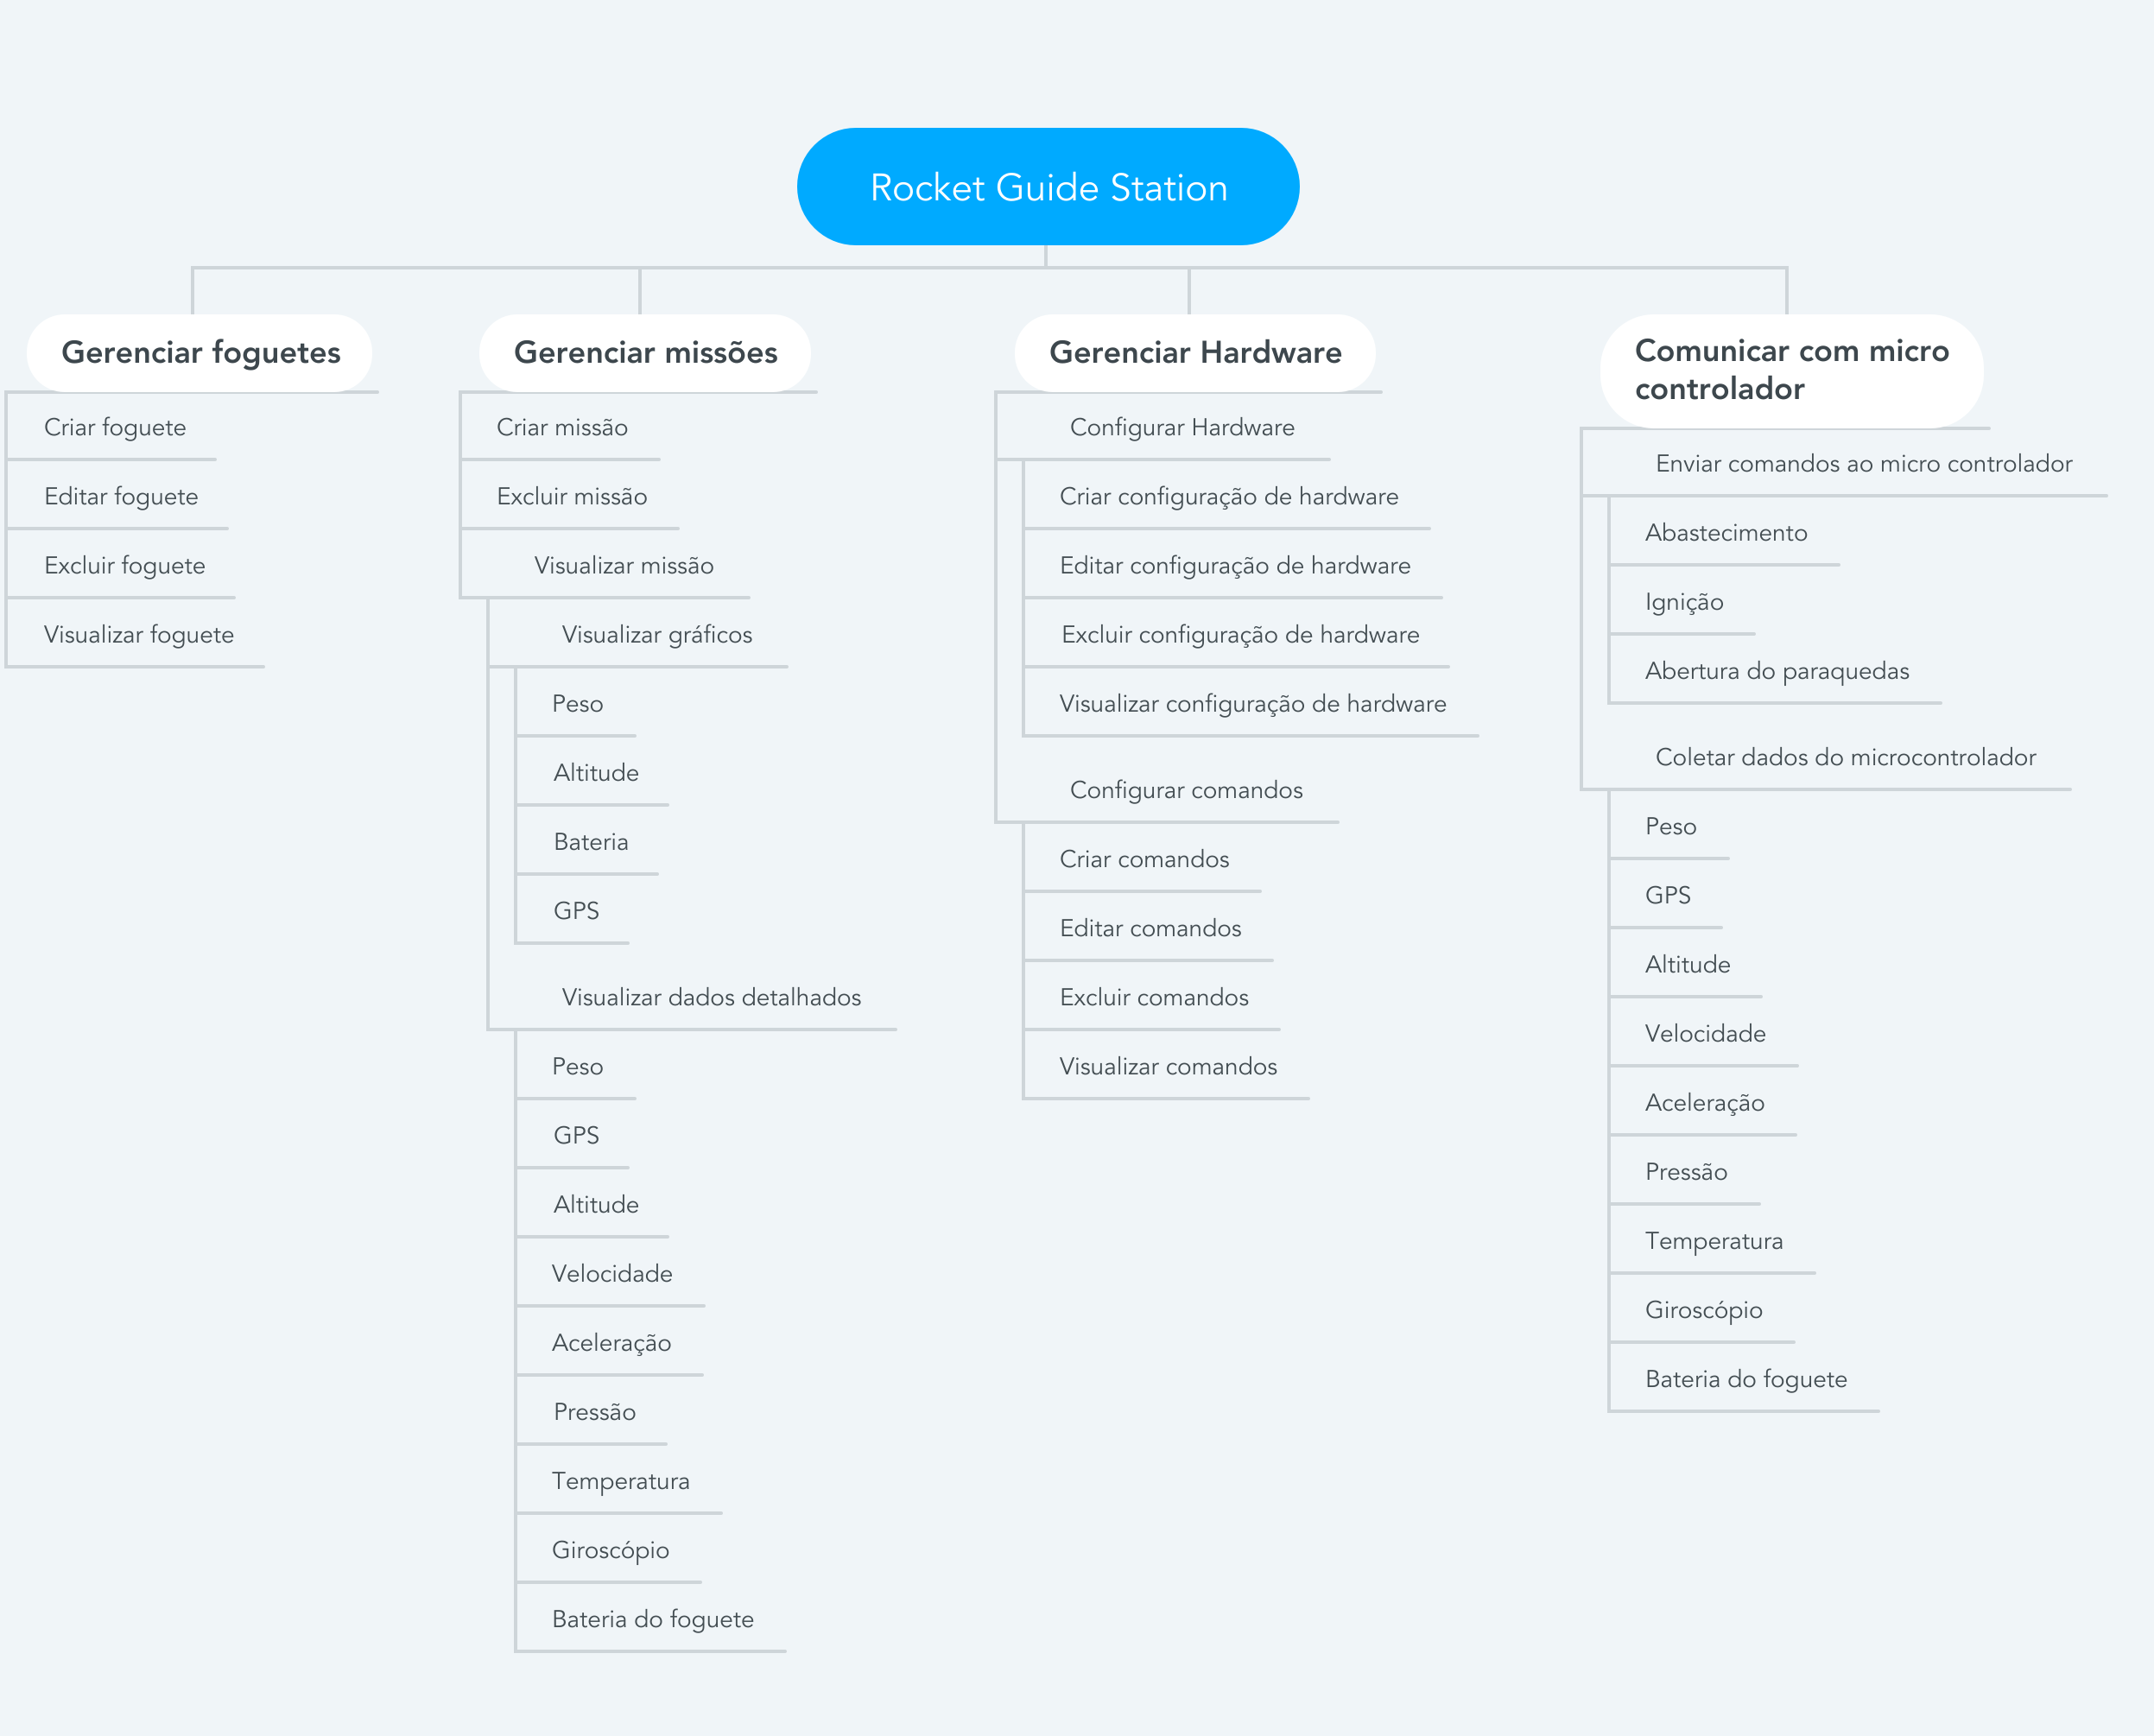
\includegraphics[scale=0.18]{figuras/Rocket_Guide_Station.png}  
\caption{Mapa de requisitos}
\label{fig:Mindmeister}
\end{figure}

\par Neste projeto, aplicamos técnicas de mapa mental para fazer a especificações de requisitos \cite{mapamental}. Utilizamos a ferramenta \textbf{Mind Meister} para construir o mapa mental. A partir da nova definição de produto, foi feito um mapa de requisitos demonstrando todos os requisitos do projeto. A Figura \ref{fig:Mindmeister} apresenta os épicos, ou principais funcionalidades: \textbf{Gerenciar Foguetes}; \textbf{Gerenciar Missões}; \textbf{Gerenciar Hardware}; e \textbf{Comunicar com o Micro Controlador}. Essas informações também estão disponíveis \href{https://mm.tt/1664123184?t=VJwmqWSqXf}{aqui}.




\section{Definição da Arquitetura}


%https://miro.com/app/board/o9J_kiYMRcI=/

\subsection{Padrão Arquitetural}

\par De acordo com o problema que o projeto visa resolver, a solução técnica proposta será embasada na arquitetura REST. A arquitetura \textit{Representational State Transfer} (REST), em português Transferência Representacional de Estado, é ideal ao nosso sistema, pois ele possui baixa complexidade e necessidade de utilização dos dados em tempo e estado definidos. De acordo com \cite{microservice} em suas conclusões, um sistema nem sempre se encaixa no perfil de um arquitetura distribuída, como a arquitetura micros-serviços, que, se aplicada de modo equivocado, pode prejudicar o bom andamento do projeto, pois exige maior complexidade no desenvolvimento e implantação do sistema, concluindo que esse tipo de arquitetura não deve ser aplicada a \textit{softwares} simples e com baixo grau de complexidade. 

\par A complexidade de um sistema nada diz sobre a eficiência e eficácia deste. Nossa solução proverá uma comunicação necessária para que as regras de negócio sejam aplicadas, satisfazendo as expectativas dos usuários e clientes. Após um estudo, foi verificado que uma \textit{Application Programming Interface} (API), em português Interface de Programação de Aplicativos, que seja RESTful, ou seja, capaz de implementar a arquitetura REST, é ideal para o problema proposto. 

\par No diagrama com protocolos de comunicação entre componentes do software, Figura \ref{fig:representacao_arq}, vemos que a comunicação entre os componentes do sistema deve ser planejada de maneira sistemática, e esse foi o caso. O sistema será construído usando a linguagem de programação JavaScript. O uso de JavaScript é bem comum para os \textit{browsers}, porém é necessários ajustes para a sua utilização a nível de \textit{backend}. Esses ajustes são realizados pelo \textit{runtime} Node.js, um ambiente em tempo de execução capaz de rodar um servidor \textit{web} local na porta 4200 como padrão. O Node.js, além de permitir a execução de código localmente fora no navegador, é responsável também por gerenciar pacotes e empacotar tudo que é necessário para executar e interpretar código JavaScript.

\par Na Figura \ref{fig:javascript backend} vê-se a lógica por trás da aplicação da linguagem \textit{JavaScript} em nossa API.

\begin{figure}[h!]
	\centering
	\label{javascript backend}
		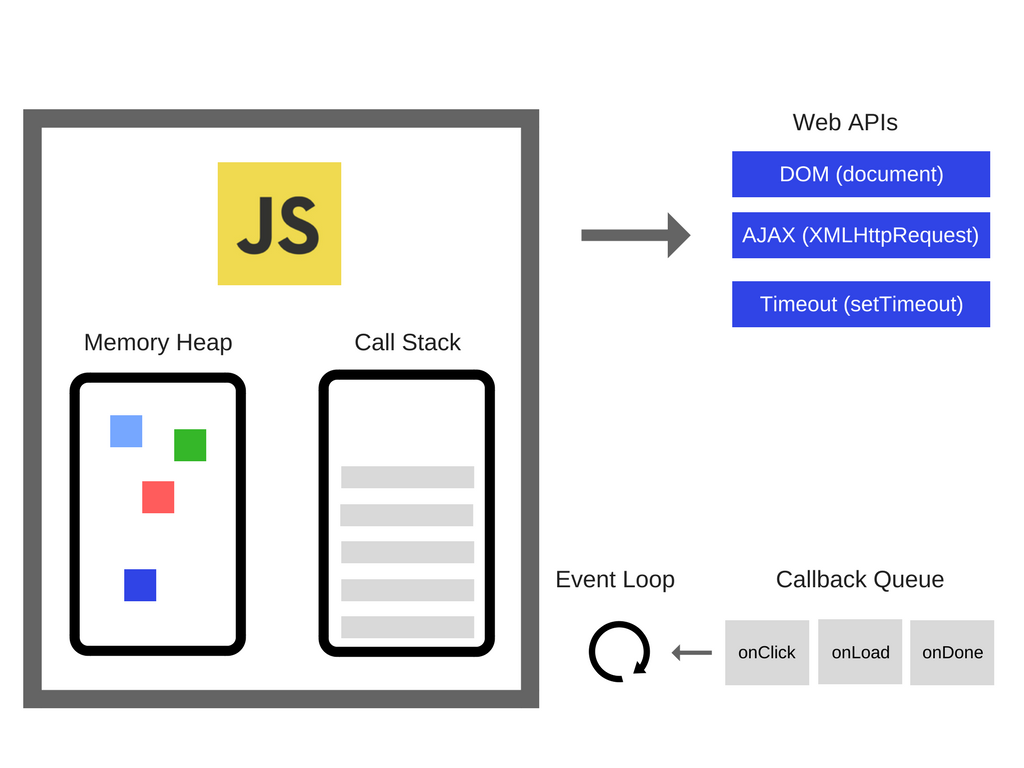
\includegraphics[keepaspectratio=true,scale=0.6]{figuras/javascript-backend.png}
	\caption{Modo como o JavaScript é executado fora do browser}
	{\footnotesize Fonte: \cite{javascript-backend}}
	\label{fig:javascript backend}
\end{figure}



\subsection{Representação da Arquitetura}

\begin{figure}[H]
\centering
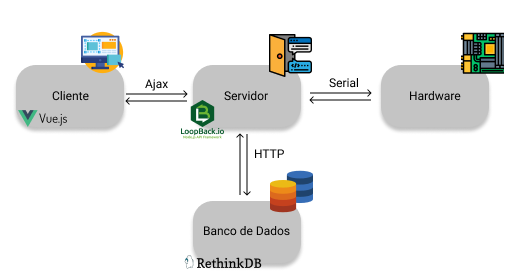
\includegraphics[width=0.9\textwidth]{figuras/representacao_arq.png}
\caption{Representação da Arquitetura}
\label{fig:representacao_arq}
\end{figure}


\subsubsection{Cliente}

\par Em aplicações \textit{web}, é muito comum adotar o conceito de \textit{Client-side} e \textit{Server-side} dentro da arquitetura em camadas \cite{ServerAndClient}. Nossa aplicação não será essencialmente \textit{web}, já que não será possível executar um \textit{browser} e também ter acesso à internet, assim como citado na Seção \ref{metas_restricoes} deste documento. Porém, vamos usar uma tecnologia inovadora implementada pelo \textit{framework} JavaScript Electron.js, que possibilita o desenvolvimento de aplicações \textit{desktop cross-platform}, em português seria algo como uma mescla de tipos de plataformas (\textit{web} e \textit{desktop}), utilizando ferramentas \textit{web} como JavaScript, HTML e CSS \cite{electron}.

\par O ciclo de vida do lado do Cliente (\textit{Client-side}) é representado na Figura \ref{fig:client-side}. O JavaScript faz requisições, ações que o usuário deseja executar ao utilizar a interface da aplicação, por meio de chamadas AJAX (Asynchronous JavaScript And XML), em português seria algo como JavaScript assíncrono + XML \cite{Ajax}. Com essa tecnologia, uma aplicação \textit{web} é capaz de realizar atualizações incrementais na interface apresentada ao usuário.

\begin{figure}[!h]
	\centering
		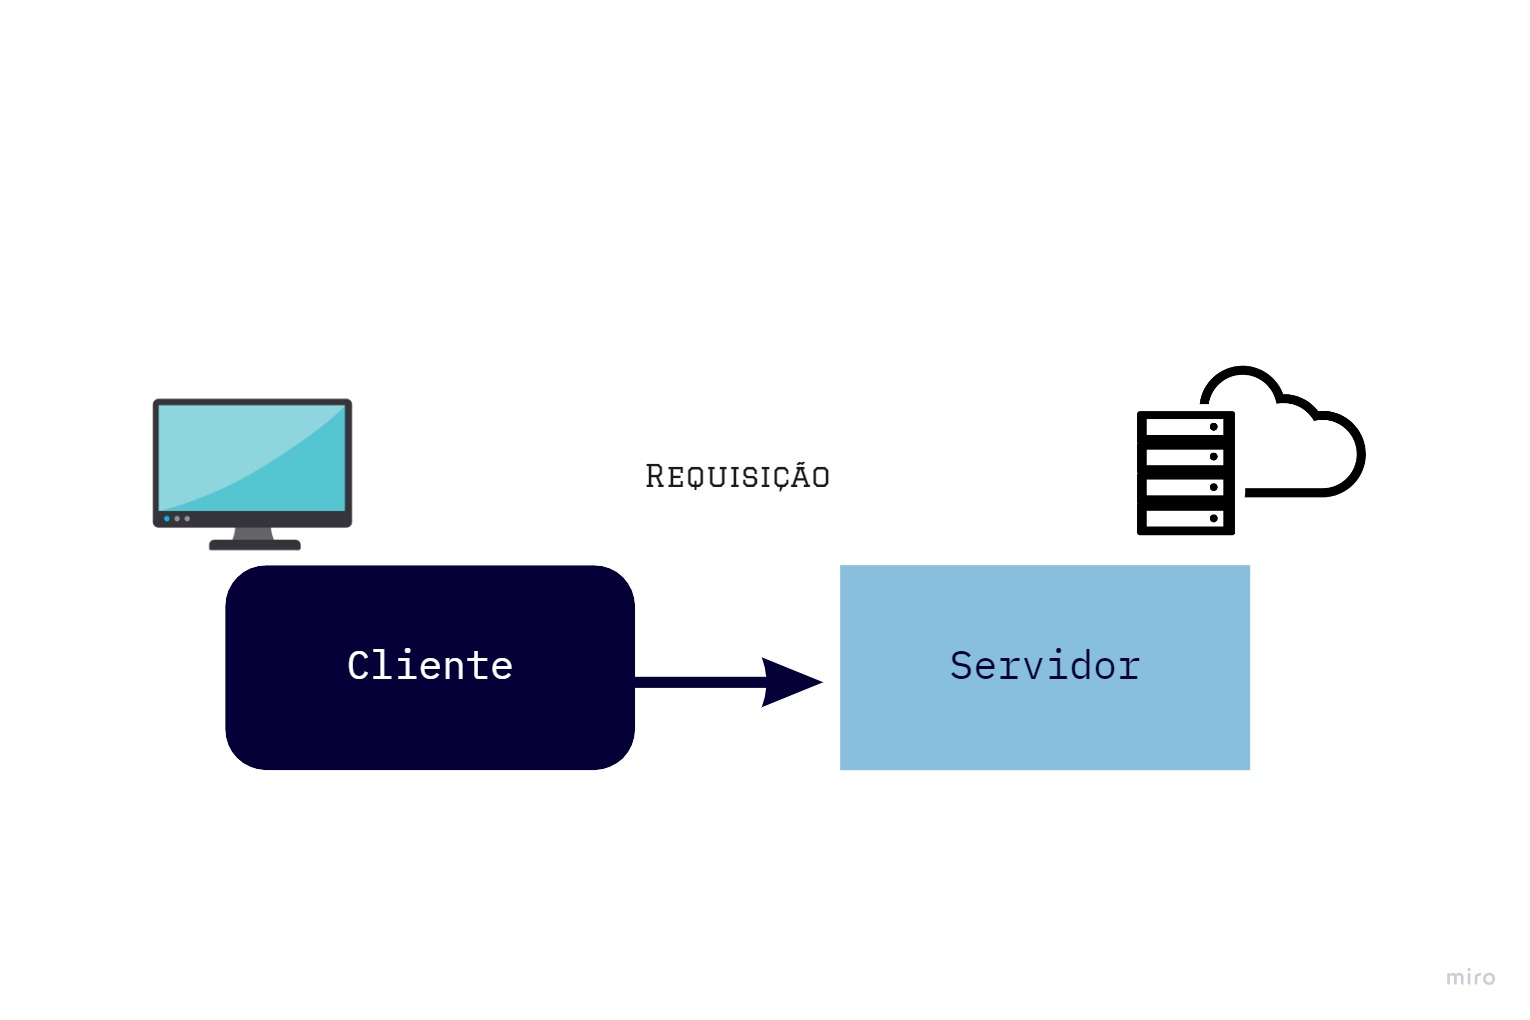
\includegraphics[keepaspectratio=true,scale=0.26]{figuras/client.jpg}
	\caption{Cliente da aplicação Desktop}
	\label{fig:client-side}
\end{figure}


\par A tecnologia que será usada é o Vue.js um \textit{progressive framework}, em português "\textit{framework} progressivo", em JavaScript para o desenvolvimento no \textit{Client-side} \cite{Vue} e também fazendo uso do "axios" que é um cliente HTTP baseado em \textit{promises}, que é um objeto usado para processamento assíncrono \cite{Promise}. Nesse contexto, o desenvolvimento \textit{frontend} será responsável por criar a interface gráfica e também a comunicação entre \textit{Client-side} e \textit{Server-side}. 

\subsubsection{Servidor}

\par Do lado do servidor, \textit{Server-side} Figura \ref{fig:Server-side}, temos recebimento de requisições por parte do cliente, o processamento lógico e, por fim, o envio da resposta correspondente ao cliente. 

\begin{figure}[H]
	\centering
		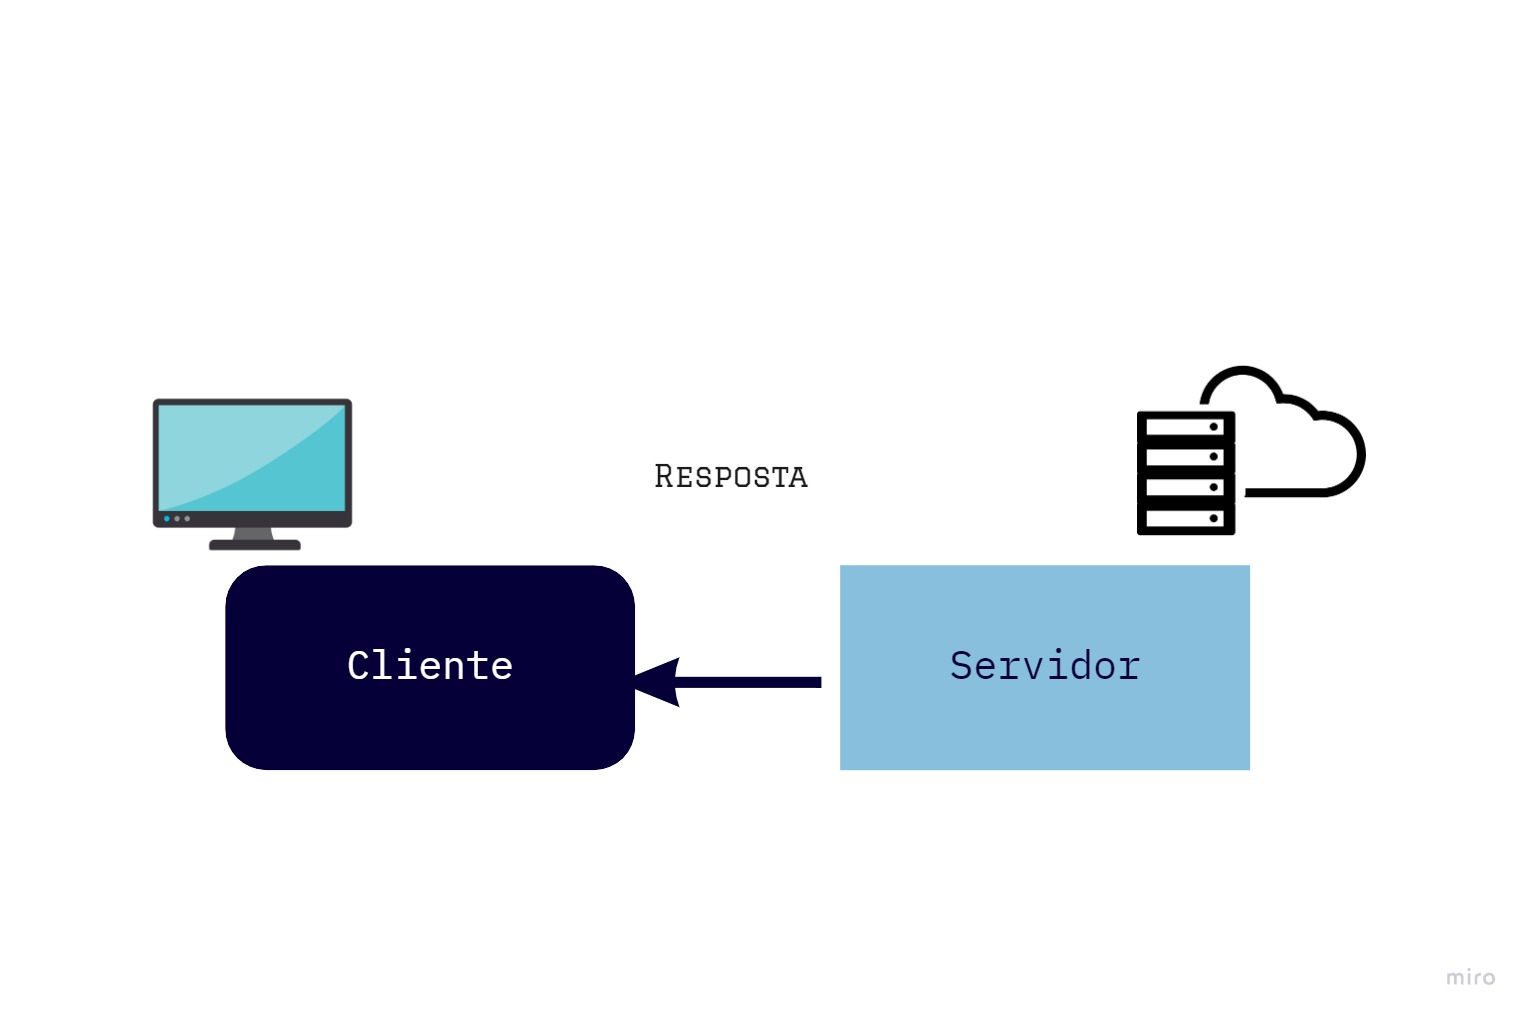
\includegraphics[keepaspectratio=true,scale=0.26]{figuras/server.jpg}
	\caption{Servidor da aplicação Desktop}
	\label{fig:Server-side}
\end{figure}

\par Faremos uso de uma API Rest escrita em JavaSript, por meio do Framework Loopback, um \textit{framework} altamente expansível baseado no famoso Express e em Node.js + Typescript \cite{Loopback}. Dessa forma, poderemos criar serviços REST que serão consumidos pelo Cliente por meio de \textit{endpoints}.

\par Para o \textit{pipeline} de funções que manipulam as requisições e respostas HTTP que serão necessárias para a comunicação com o Banco de dados, faremos o uso de \textit{middleware}. Esse tipo de metodologia de processamento implementa o padrão de projeto \textit{Chain of Responsability}  \cite{Chain}, o qual é desenhado para desacoplar o envio e recebimento de mensagens dividindo a tarefa de manipulá-las entre múltiplos objetos tal como na Figura \ref{fig:chain-of-responsibility}.

\begin{figure}[H]
	\centering
	\label{chain-of-responsibility}
		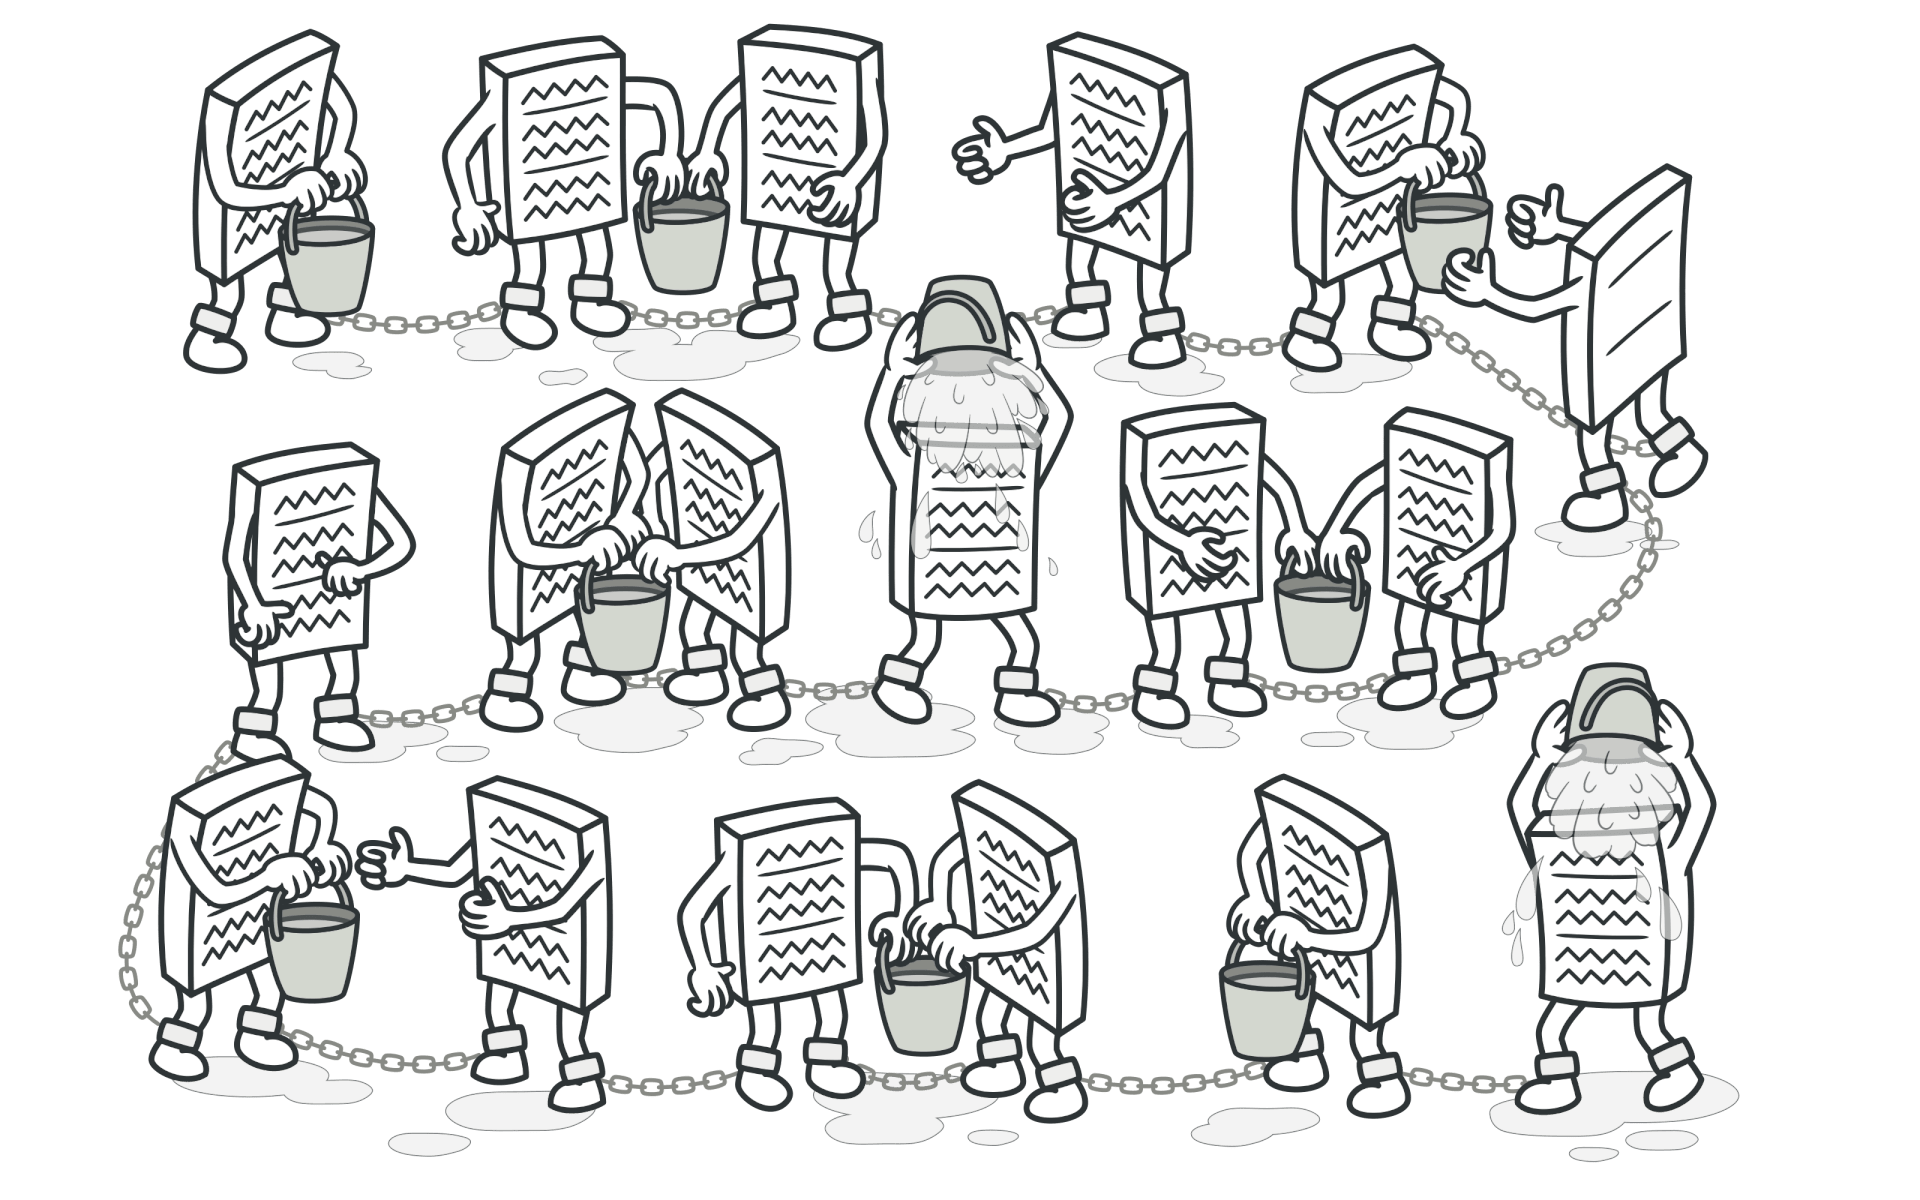
\includegraphics[keepaspectratio=true,scale=0.22]{figuras/chain-of-responsibility.png}
	\caption{Padrão de Projeto Chain of Responsability \cite{ChainFigura}}
	\label{fig:chain-of-responsibility}
\end{figure}

\par Com o \textit{Loopback}, podemos criar uma sequencia de funções que realizam o processamento adequado de mensagens conforme representado na Figura \ref{fig:middleware} \cite{Loopback}.

\begin{figure}[H]
	\centering
	\label{middleware}
		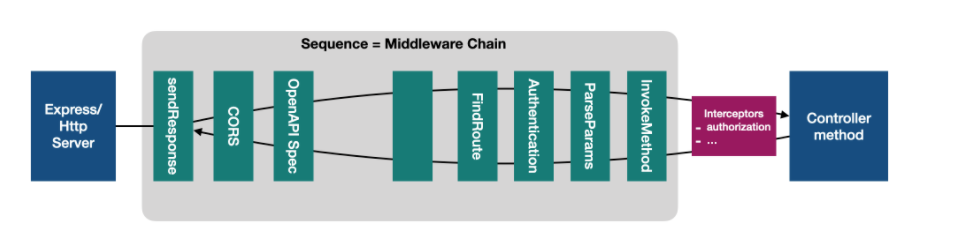
\includegraphics[keepaspectratio=true,scale=0.75]{figuras/middleware.png}
	\caption{Sequência baseada em Middleware  \cite{Loopback}}
	\label{fig:middleware}
\end{figure}


\subsubsection{Banco de Dados}

\par Para oferecer uma experiência satisfatória ao usuário da aplicação, os dados devem ser apresentados em tela em tempo real. Nossa base de dados deve ser capaz de detectar qualquer mudança realizada em seu armazenamento. Para isso, optamos por usar a tecnologia do banco de dados RethinkDB, um banco de dados \textit{open-source} capaz de realizar envio de dados no formato JSON em tempo real. 

\par Além disso, é um banco de dados NoSQL, que nos permite flexibilidade se comparado com bancos SQL, mas que mantém a organização a nível de modelagem de dados. A tecnologia por trás disso é a \textit{schemaless JSON documents}, um armazenamentos de documentos JSON não esquematizado.Todos os documentos NoSQL armazenam suportam as mesmas operações básicas:

\begin{itemize}
    \item criar ou apagar registros de uma coleção;
    \item criar, recuperar, atualizar ou deletar um documento;
    \item consultar uma coleção;
    \item criar ou apagar registros de índices. 
\end{itemize}

\par Dessa forma, teremos uma ferramenta poderosa para manipular nossos dados.Diferentemente de bancos SQL, os arquivos são escritos em documentos, com estruturas semelhantes às Figuras \ref{fig:json} e \ref{fig:xml}.

\begin{figure}[!h]
	\centering
	\label{json}
		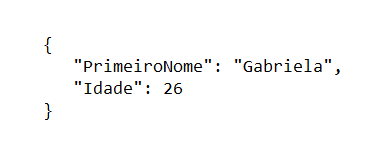
\includegraphics[keepaspectratio=true,scale=0.9]{figuras/json.png}
	\caption{Documento em formato JSON}
	\label{fig:json}
\end{figure}

\begin{figure}[!h]
	\centering
	\label{xml}
		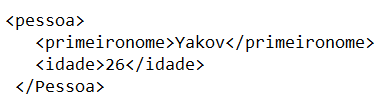
\includegraphics[keepaspectratio=true,scale=0.9]{figuras/xml.png}
	\caption{Documento em formato XML}
	\label{fig:xml}
\end{figure}

\subsubsection{\textit{Hardware}}

\par A comunicação entre o \textit{hardware} e o \textit{software} do projeto é feita via porta serial. Em fase experimental, iremos fazer um \textit{script} para simular o funcionamento dessa integração e relatar o desempenho possível e desejado. Até o momento, não foram encontradas evidências de que o \textit{script} não poderá ser escrito em JavaScript, já que existe a biblioteca Serialport.js \cite{serialport} que dá o necessário suporte a esse tipo de comunicação. Porém, caso haja qualquer problema de compatibilidade, faremos uso do padrão de projeto Adaper, que tem como objetivo prover uma interface que liga objetos com diferentes tipos de linguagem e protocolos de comunicação. O padrão é representado pela Figura \ref{fig:adapter}.

\begin{figure}[!h]
	\centering
	\label{adapter}
		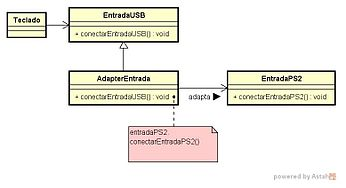
\includegraphics[keepaspectratio=true,scale=1]{figuras/adapter.jpg}
	\caption{Padrão de projeto Adapter \cite{Adapter}}
	\label{fig:adapter}
\end{figure}

\subsection{Ambiente}

\par Tendo em vista a arquitetura do projeto e a falta da placa para testar o sistema nas condições reais, foi adotada a estratégia de conteinerização dos serviços. Assim é possível isolar os ambientes, bem como facilitar a configuração do ambiente de produção (já embarcado no dispositivo). Para isso, foram utilizadas as seguintes tecnologias:

\begin{itemize}
    \item Docker \cite{docker}
    \item Docker - Compose \cite{docker-compose}
\end{itemize}

\subsection{Arquitetura computacional}

\par O sistema será desenvolvido para ser executado em um computador de arquitetura 64 bit ARM (Arm64) e um sistema operacional que opere nessa mesma arquitetura \cite{arquitetura_arm}.

\section{Diagrama de Sequência}

\par O principal objetivo do diagrama de sequência é verificar se ele é consistente com a declaração dos requisitos, bem como com sua estrutura de árvore bem formada. Enquanto isso, a construção do diagrama é definida em termos das transições de estado, que são realizadas pelas invocações de método no diagrama, representados no nosso contexto por Cliente, Servidor, Banco de Dados e Micro Controlador. Quando uma mensagem é executada, ela deve ser consistente com o estado do sistema, e com as dependências de transações entre os estados \cite{li2004formal}.

\par Para garantir um alinhamento e uma comunicação de qualidade com os componentes de eletrônica, esse diagrama foi evoluído para garantir a documentação e a estruturação da comunicação entre os times. A Figura \ref{fig:Diagrama_sequencia_missao_1} apresenta a fase de missão, onde o usuário solicita o início da ignição à camada da interface, que por sua vez, solicita ao servidor (camada da API), que consulta o comando a ser enviado ao hardware no banco de dados, e ao obter essa informação envia o comando. Após receber o comando e iniciar o processo, o sistema receberá uma confirmação do início. Após confirmar o início do processo de ignição, é realizada a troca da comunicação que antes era feita com o microcontrolador da base e que agora será feita com o do foguete, para receber as informações do voo. A atualização das informações para o usuário é iniciada em um loop, como apresentado no Apêndice \ref{diagrama_sequencia}, Figura \ref{fig:Diagrama_sequencia_missao}. Que apresenta o loop que é executado durante todo o processo para coletar as informações dos sensores e armazenar no banco de dados. As Figuras \ref{fig:Diagrama_sequencia_cadastr_foguete}, \ref{fig:Diagrama_sequencia_cadastro_micro}, \ref{fig:Diagrama_sequencia_missao}, \ref{fig:Diagrama_sequencia_abastecimento}, \ref{fig:Diagrama_sequencia_desengate}, \ref{fig:Diagrama_sequencia_ignicao}, \ref{fig:Diagrama_sequencia_finaliza_missao}, \ref{fig:Diagrama_sequencia_historico} apresentam respectivamente o processo de lançamento do foguete pela estação desenvolvida.

\begin{figure}[htb]
    \centering
    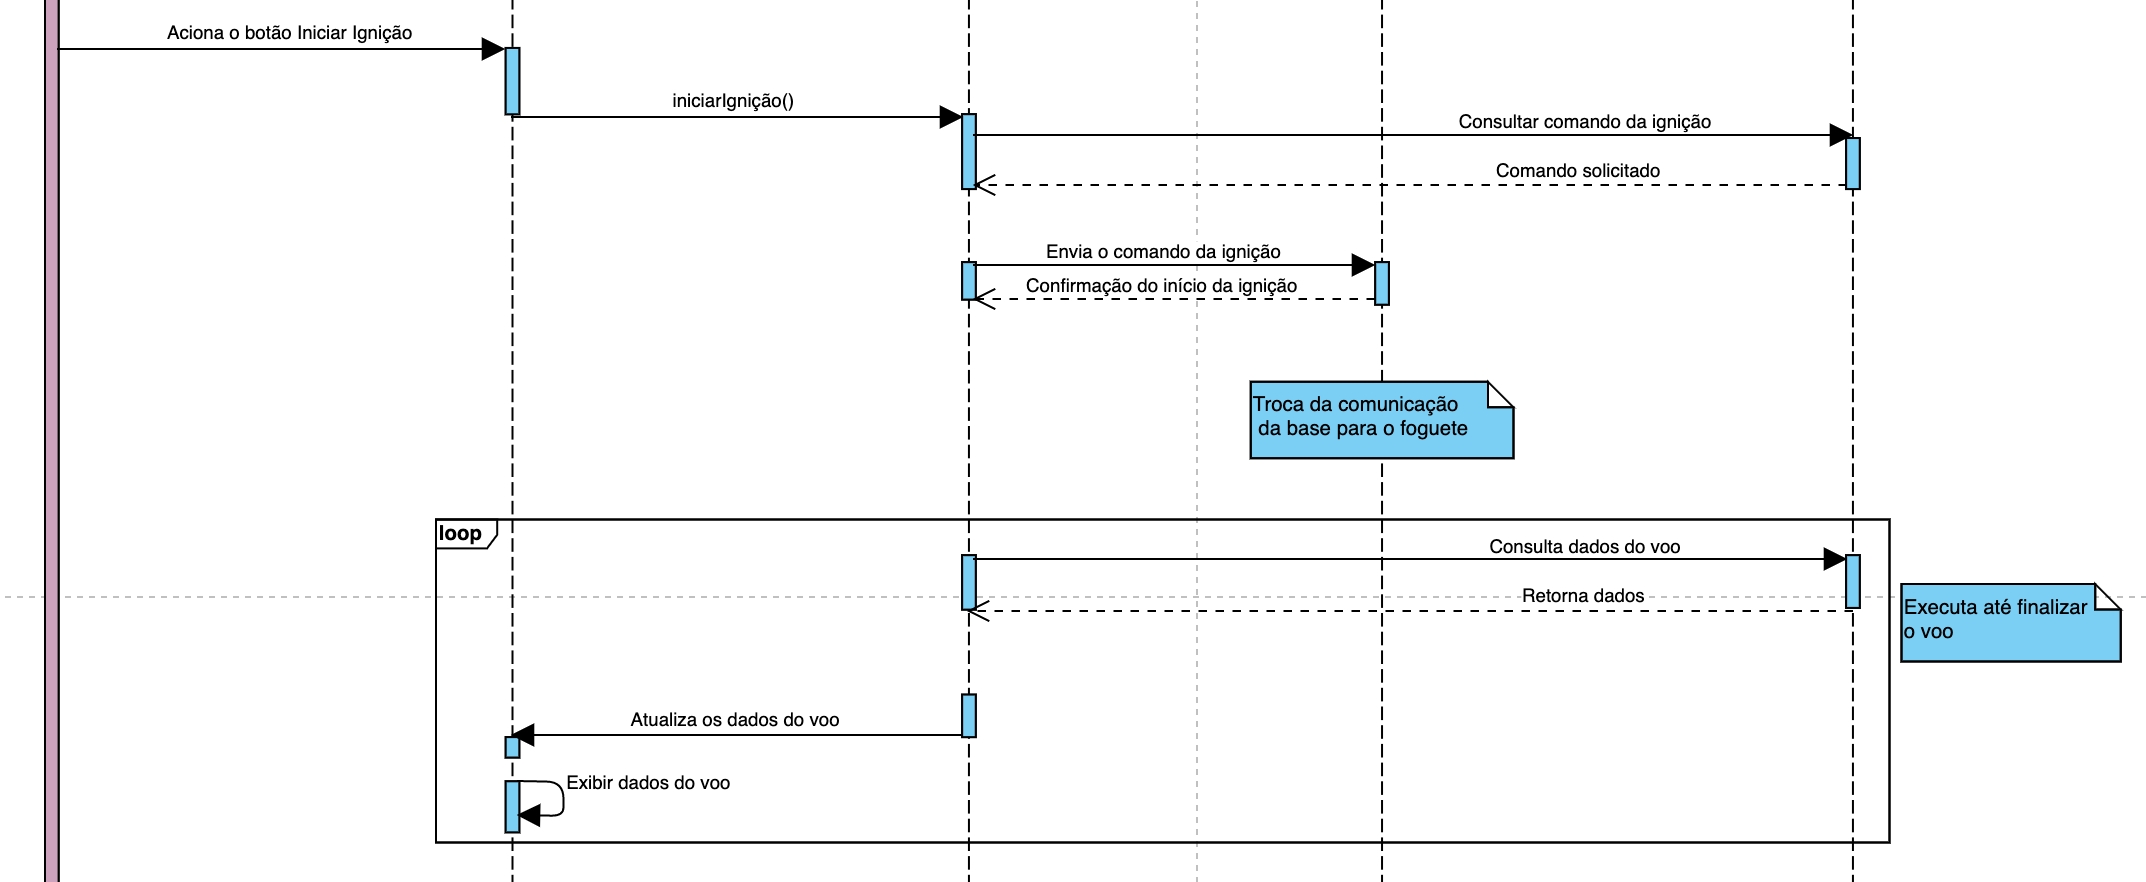
\includegraphics[width=1\textwidth, angle=0]{figuras/diagrama_sequencia_ignicao.png}
    \caption{Diagrama de sequencia representando o processo da ignição do foguete. Fonte: Autor}
    \label{fig:Diagrama_sequencia_missao_1}
\end{figure}

\par Nós construímos o diagrama de sequência, presente no Apêndice \ref{diagrama_sequencia}, com o objetivo de alinhar o processo de lançamento e especificar os requisitos.

\section{Modelagem de Dados}

\par A modelagem dos dados foi feita com base nos requisitos e utilizando o \textit{software} BrModelo. Primeiro, optamos por fazer o modelo conceitual especificar em um nível mais alto as entidades e seus relacionamentos. A Figura \ref{fig:conceitual} apresenta as entidades: \textbf{Foguete, Missão, Temperatura, Velocidade, GPS e Pressão}, mantendo um relacionamento. As entidades \textbf{Hardware e Comando} não possuem relação com a entidade Foguete e Comando, pois se trata de uma configuração presente na \textit{Ground Station} apenas, não interagindo assim diretamente na Missão e no funcionamento do Foguete.

\begin{figure}[h!]
	\centering
		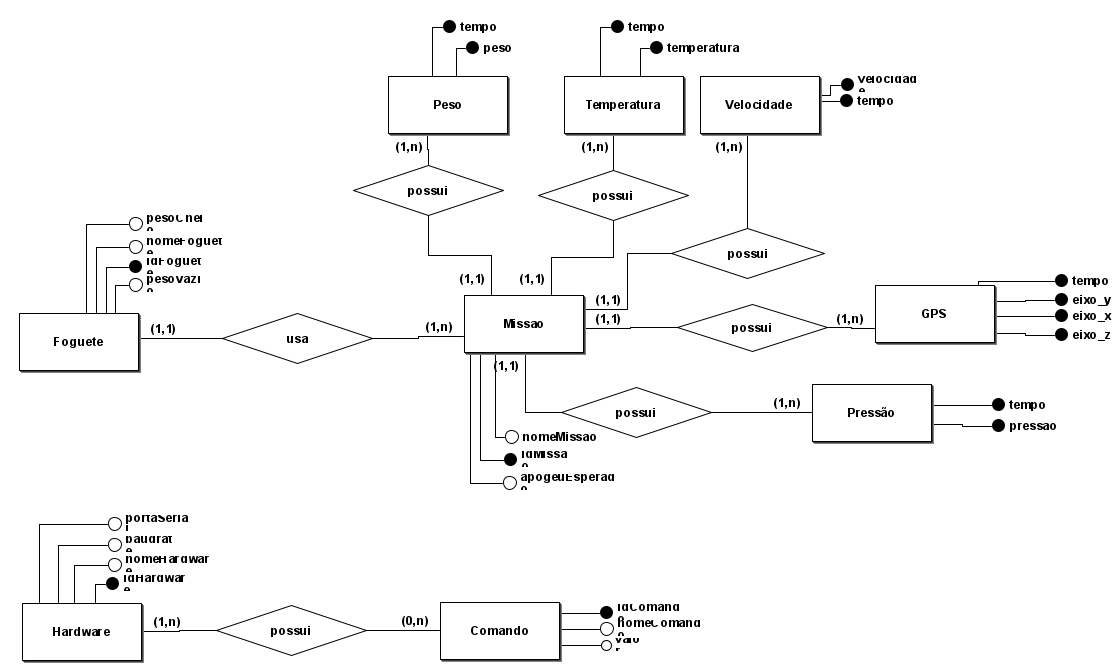
\includegraphics[keepaspectratio=true,scale=0.4]{figuras/conceitual_ground_station.png}
	\caption{Modelo Conceitual da modelagem.}
	\label{fig:conceitual}
\end{figure}


\begin{figure}[h!]
	\centering
		\includegraphics[keepaspectratio=true,scale=0.4]{figuras/Lógico_ground_station.png}
	\caption{Modelo Lógico da modelagem}
	\label{fig:logico}
\end{figure}

\par Em seguida, foi gerado o modelo lógico da implementação para representar as tabelas junto com as chaves primarias e estrangeiras. A Figura \ref{fig:logico} apresenta essa implementação.

\section{Diagrama de Pacotes}
A Figura \ref{fig:diagrama_pacote_backend} apresenta o diagrama de pacotes do backend do projeto. Ele contem a estrutura de pastas utilizada para o desenvolvimento utilizando loopback4.js. Essa estrutura apresenta as pastas e as relações entre elas para a o funcionamento do projeto.
\begin{figure}[h!]
	\centering
		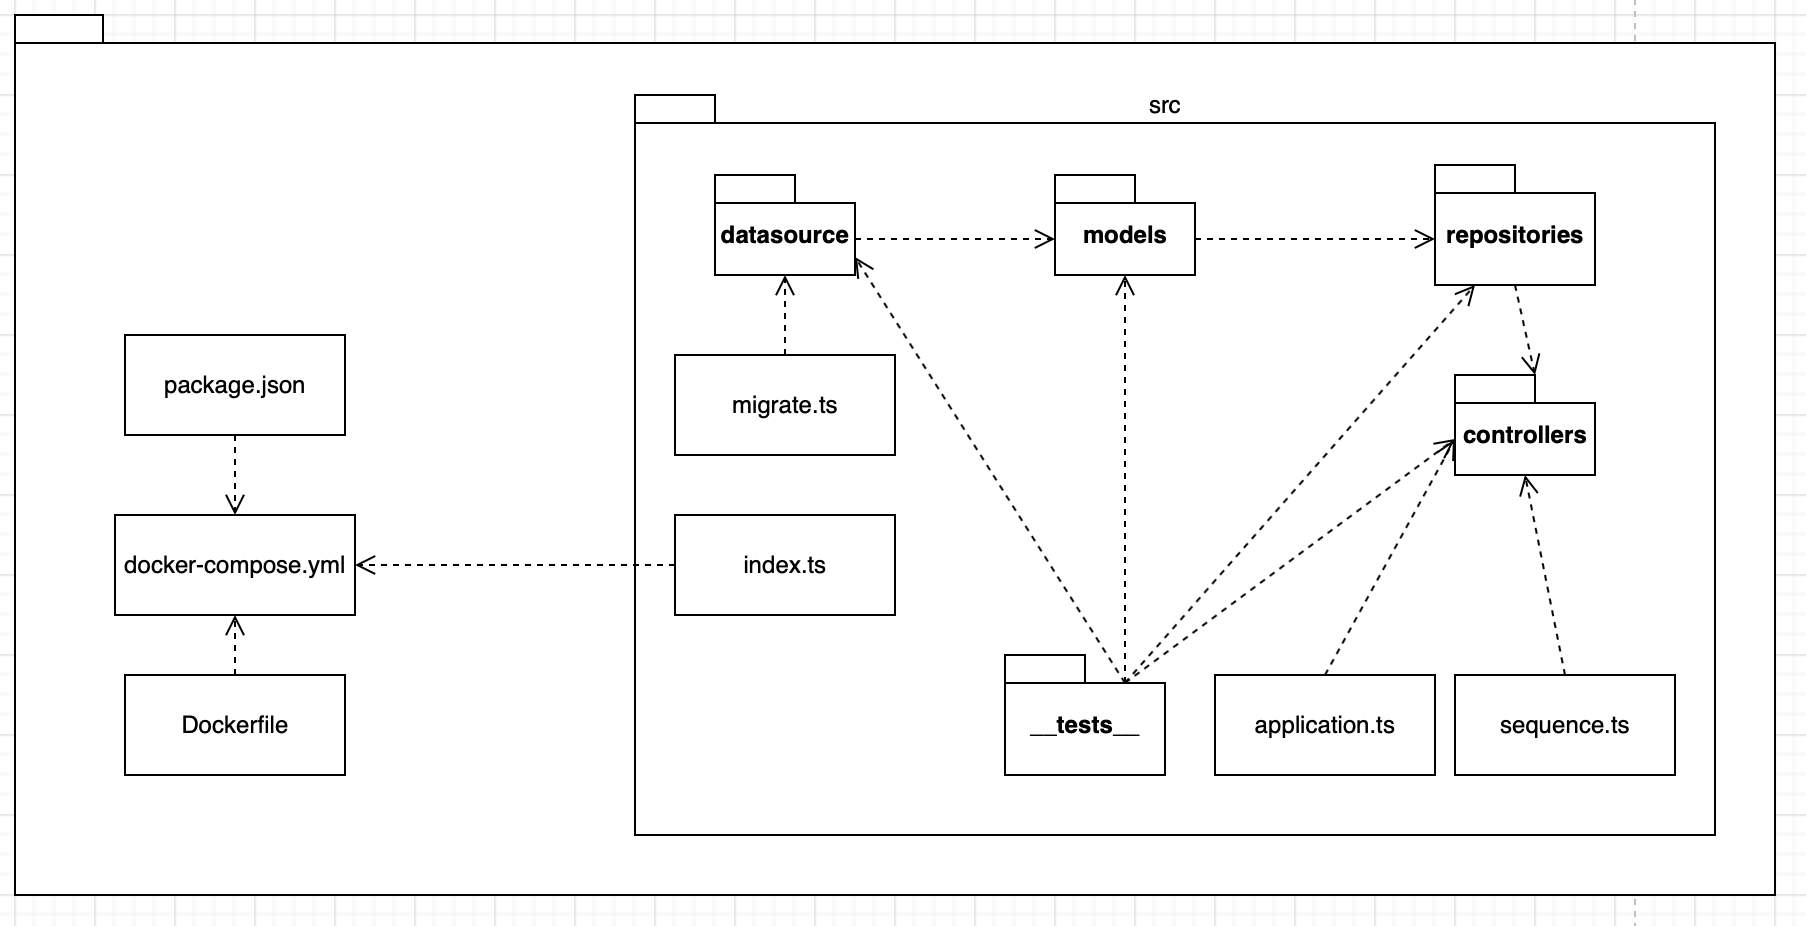
\includegraphics[keepaspectratio=true,scale=0.4]{figuras/diagrama_pacotes_backend.png}
	\caption{Diagrama de representação dos pacotes e as relações do Back end}
	\label{fig:diagrama_pacote_backend}
\end{figure}

A Figura \ref{fig:diagrama_pacote_frontend} apresenta a organização de pacotes do front end a partir de um diagrama de pacotes. O Vue.js é organizado de uma forma em que os arquivos das \textit{Views} e das \textit{Models}, representado pela pasta \textit{Store}. Além disso, o Vue permite a criação de componentes, que ficam armazenados na pasta \textit{Components} e podem ser utilizados em páginas das \textit{Views}.
\begin{figure}[h!]
	\centering
		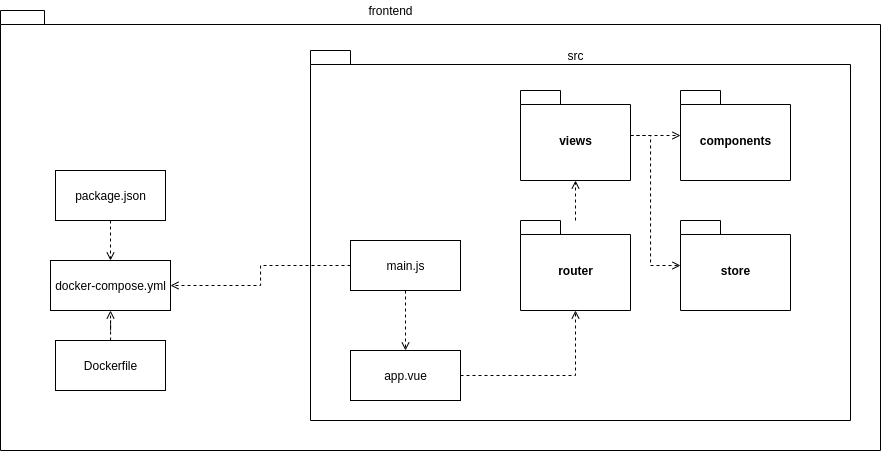
\includegraphics[keepaspectratio=true,scale=0.4]{figuras/diagrama_pacotes_frontend.png}
	\caption{Diagrama de representação dos pacotes e as relações do Front end}
	\label{fig:diagrama_pacote_frontend}
\end{figure}

\section{Metas e restrições de arquitetura}
\label{metas_restricoes}

\subsection{Metas}

\begin{itemize}
    \item Auxiliar o usuário no lançamento e acompanhamento de voo de um foguete experimental.
    \item Armazenar dados dos lançamentos de forma sistemática.
    \item Ter uma interface intuitiva e de fácil utilização, para agilizar o processo de lançamento do foguete e análise dos dados pós voo.
    \item Possibilitar o controle do lançamento e acompanhamento do voo do foguete.
\end{itemize}

\subsection{Restrições}

\begin{itemize}
    \item O sistema não terá acesso a internet.
    \item Deve ser executado em microcomputador com recursos limitados.
    \item Realizar  \textit{streaming} de dados obtidos do foguete em tempo de execução.
    \item Disponibilizar dados armazenados em CSV para exportação via cartão SD.
    \item Utilizar ambiente conteinerizado, Docker, para virtualização do ambiente, a fim de poder simular o comportamento do software, já que não teremos a placa para fazer os testes.
    \item Deve ser utilizado um computador de arquitetura 64 bit ARM, Arm64, e um sistema operacional compatível.
\end{itemize}

\section{Inovação}
Como proposta de inovação, foi definida pela equipe, que o produto seria construido com base na metodologia do \textit{User Centered Design}. Por isso, todo o processo de elaboração e construção do produto, dês da sua ideação até a sua execução foram pautados nas regras da metodologia, e com base a equipe se aprofundava na obtenção de conhecimentos relacionados ao tema, os documentos iam sendo elaborados , revisados e refinados.

\section{Descrição do problema e proposta de inovação}

O User Centered design é o processo que foca nas necessidades e desejos dos usuários para o desenvolvimento de serviços ou produtos. A aplicação consistente de fatores humanos, ergonomia, usabilidade e outras técnicas é o que permite envolver os usuários no processo de elaboração do produto, junto á equipe de desenvolvimento.

O objetivo disso é criar sistemas altamente úteis e acessíveis, apontando na direção da satisfação dos usuários, evitando efeitos negativos na performance. É colocar cada pessoa para a qual o produto foi destinado no coração da experiência.

Comumente, os produtos de estações de controle terrestres são sistemas que são construidos visando tecnicidade e com pouco foco nas demandas reais dos usuários e pouca customização para cada caso específico.Assim, o design focado no cliente pode não apenas fornecer resultados reais e mensuráveis, mas também proporcionar uma vantagem competitiva diferenciada para o produto, pois foca em ter as necessidades específicas de um nicho de usuário sanadas, baseado em suas demandas em uma construção conjunta.

\subsection{Como executar um design de produto centrado no usuário}

O processo de construção de um user centered design se divide basicamente nas quatro fases a seguir:

\begin{itemize}
    \item Análise: Essa é  a fase de pesquisa, com análise de stakeholders, competidores, desenvolvimento de personas, definição de cenários de uso, condução de estudos de campo e definição de objetivos de usabilidade. 
    \item Design: Durante o design são criados modelos de navegação, fluxos de tela, arquitetura da informação, protótipos, wireframes, design de interação (ui design) e feitos alguns testes de usuário. Todos esses processos se utilizam das informações coletadas na análise para serem feitos pensando no usuário.
    \item Implementação : Durante a implementação, é finalizado o design orientado à objetos, a integração de interfaces de design, implementação de servers e realizada constante validação com os usuários.
    \item Desenvolvimento: A parte final é a parte do desenvolvimento, onde a avaliação contínua e valudação com o usuário se transformam em produto a partir das soluções identificadas nas fases anteriores. Nessa etapa, percebe-se a importância de uma construção de produto transparente e objetiva, para que o produto desenvolvido esteja o mais próximo possível do idealizado. 
\end{itemize}

A Figura \ref{fig:ucer_centered_design_fig} apresenta o processo de ciclo de vida da metodologia User Centered Design. As etapas subsequentes foram adotadas pela equipe e ajustadas de acordo com as demandas do projeto. 

\begin{figure}[h!]
	\centering
		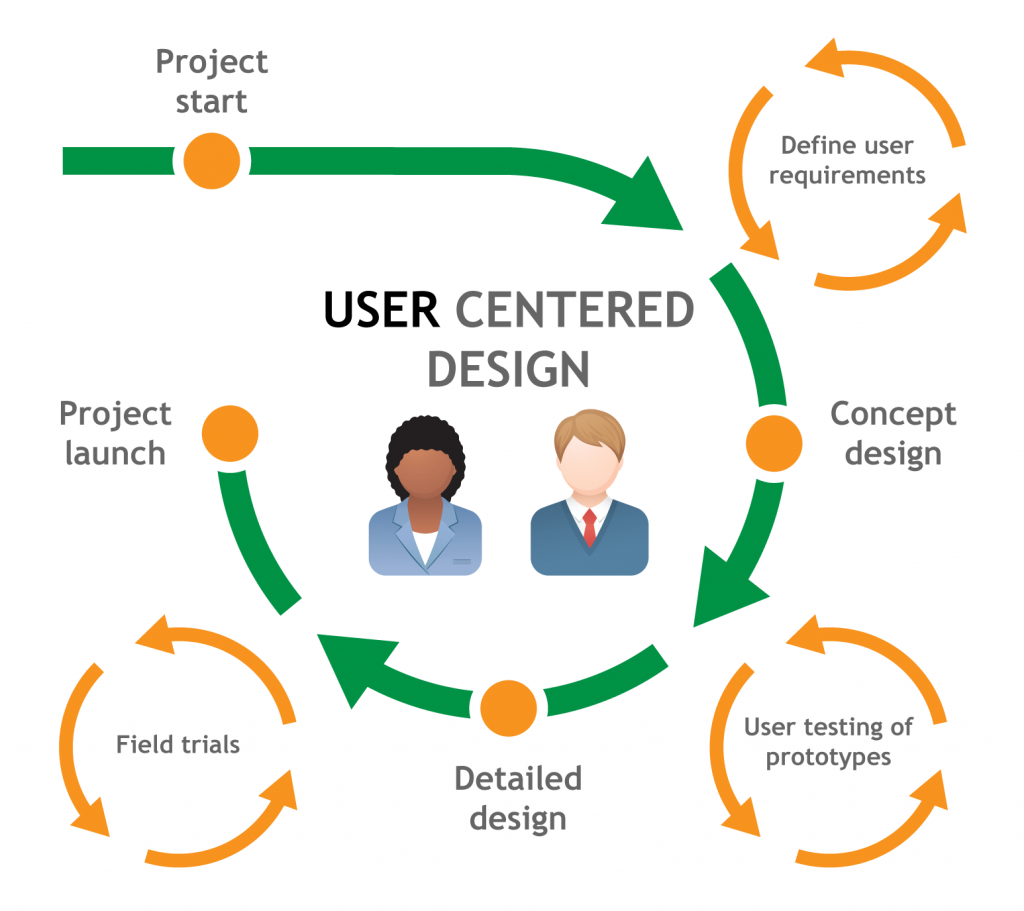
\includegraphics[keepaspectratio=true,scale=0.4]{figuras/UserCentered.png}
	\caption{Ciclo de vida do User Centered Design}
	\label{fig:ucer_centered_design_fig}
\end{figure}

\section{Construção Front end}

A construção do Front end foi desenvolvida com base no protótipo apresentado na Sessão \ref{prototipo}, utilizando vue.js. Todas as telas apresentadas à seguir foram construidas para garantir controle e monitoramento do usuário antes, durante e depois do processo de lançamento do foguete.


\subsection{Criação do Foguete}

A tela de criação do foguete, apresentada na Imagem \ref{fig:cria_foguete} é uma das primeiras a ser utilizada pelos usuários. Principalmente no primeiro uso, será necessário cadastrar um foguete, inserindo as informações de peso cheio, peso vazio e o nome do foguete. 

\begin{figure}[h!]
	\centering
		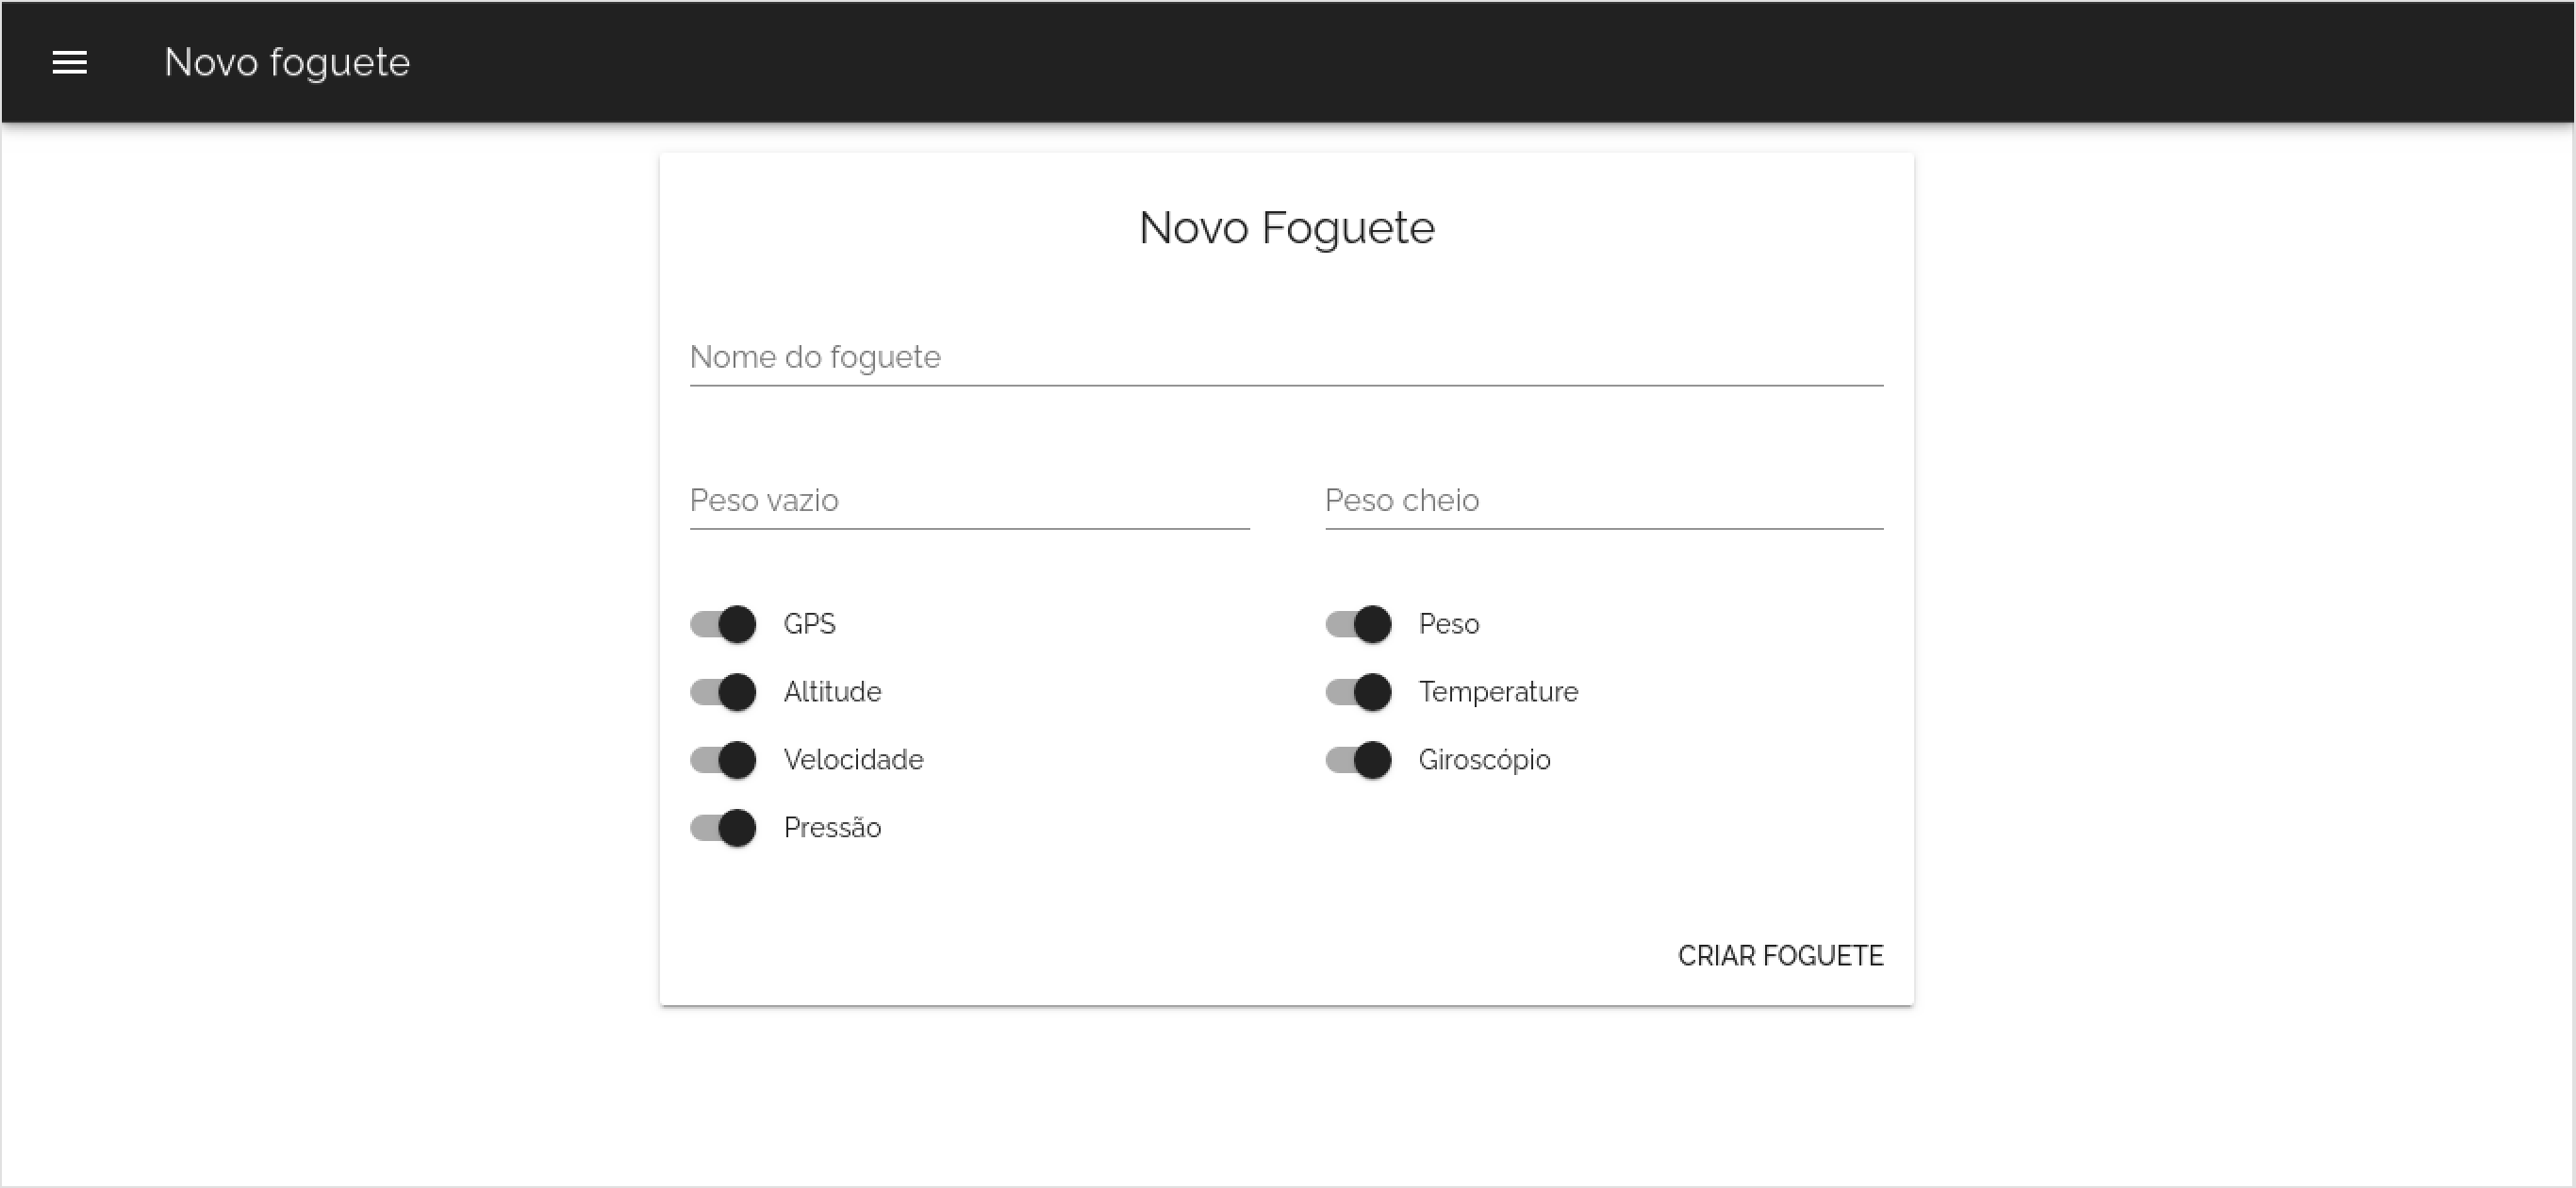
\includegraphics[keepaspectratio=true,scale=0.33]{figuras/telas_software/1.png}
	\caption{Tela de criação de foguetes.}
	\label{fig:cria_foguete}
\end{figure}

Caso o usuário deixe de informar algum dos dados obrigatórios, é feita a validação para informar e impedir que a o foguete seja criado fora dos padrões, como apresentado na Figura \ref{fig:cria_foguete_error}.

\begin{figure}[h!]
	\centering
		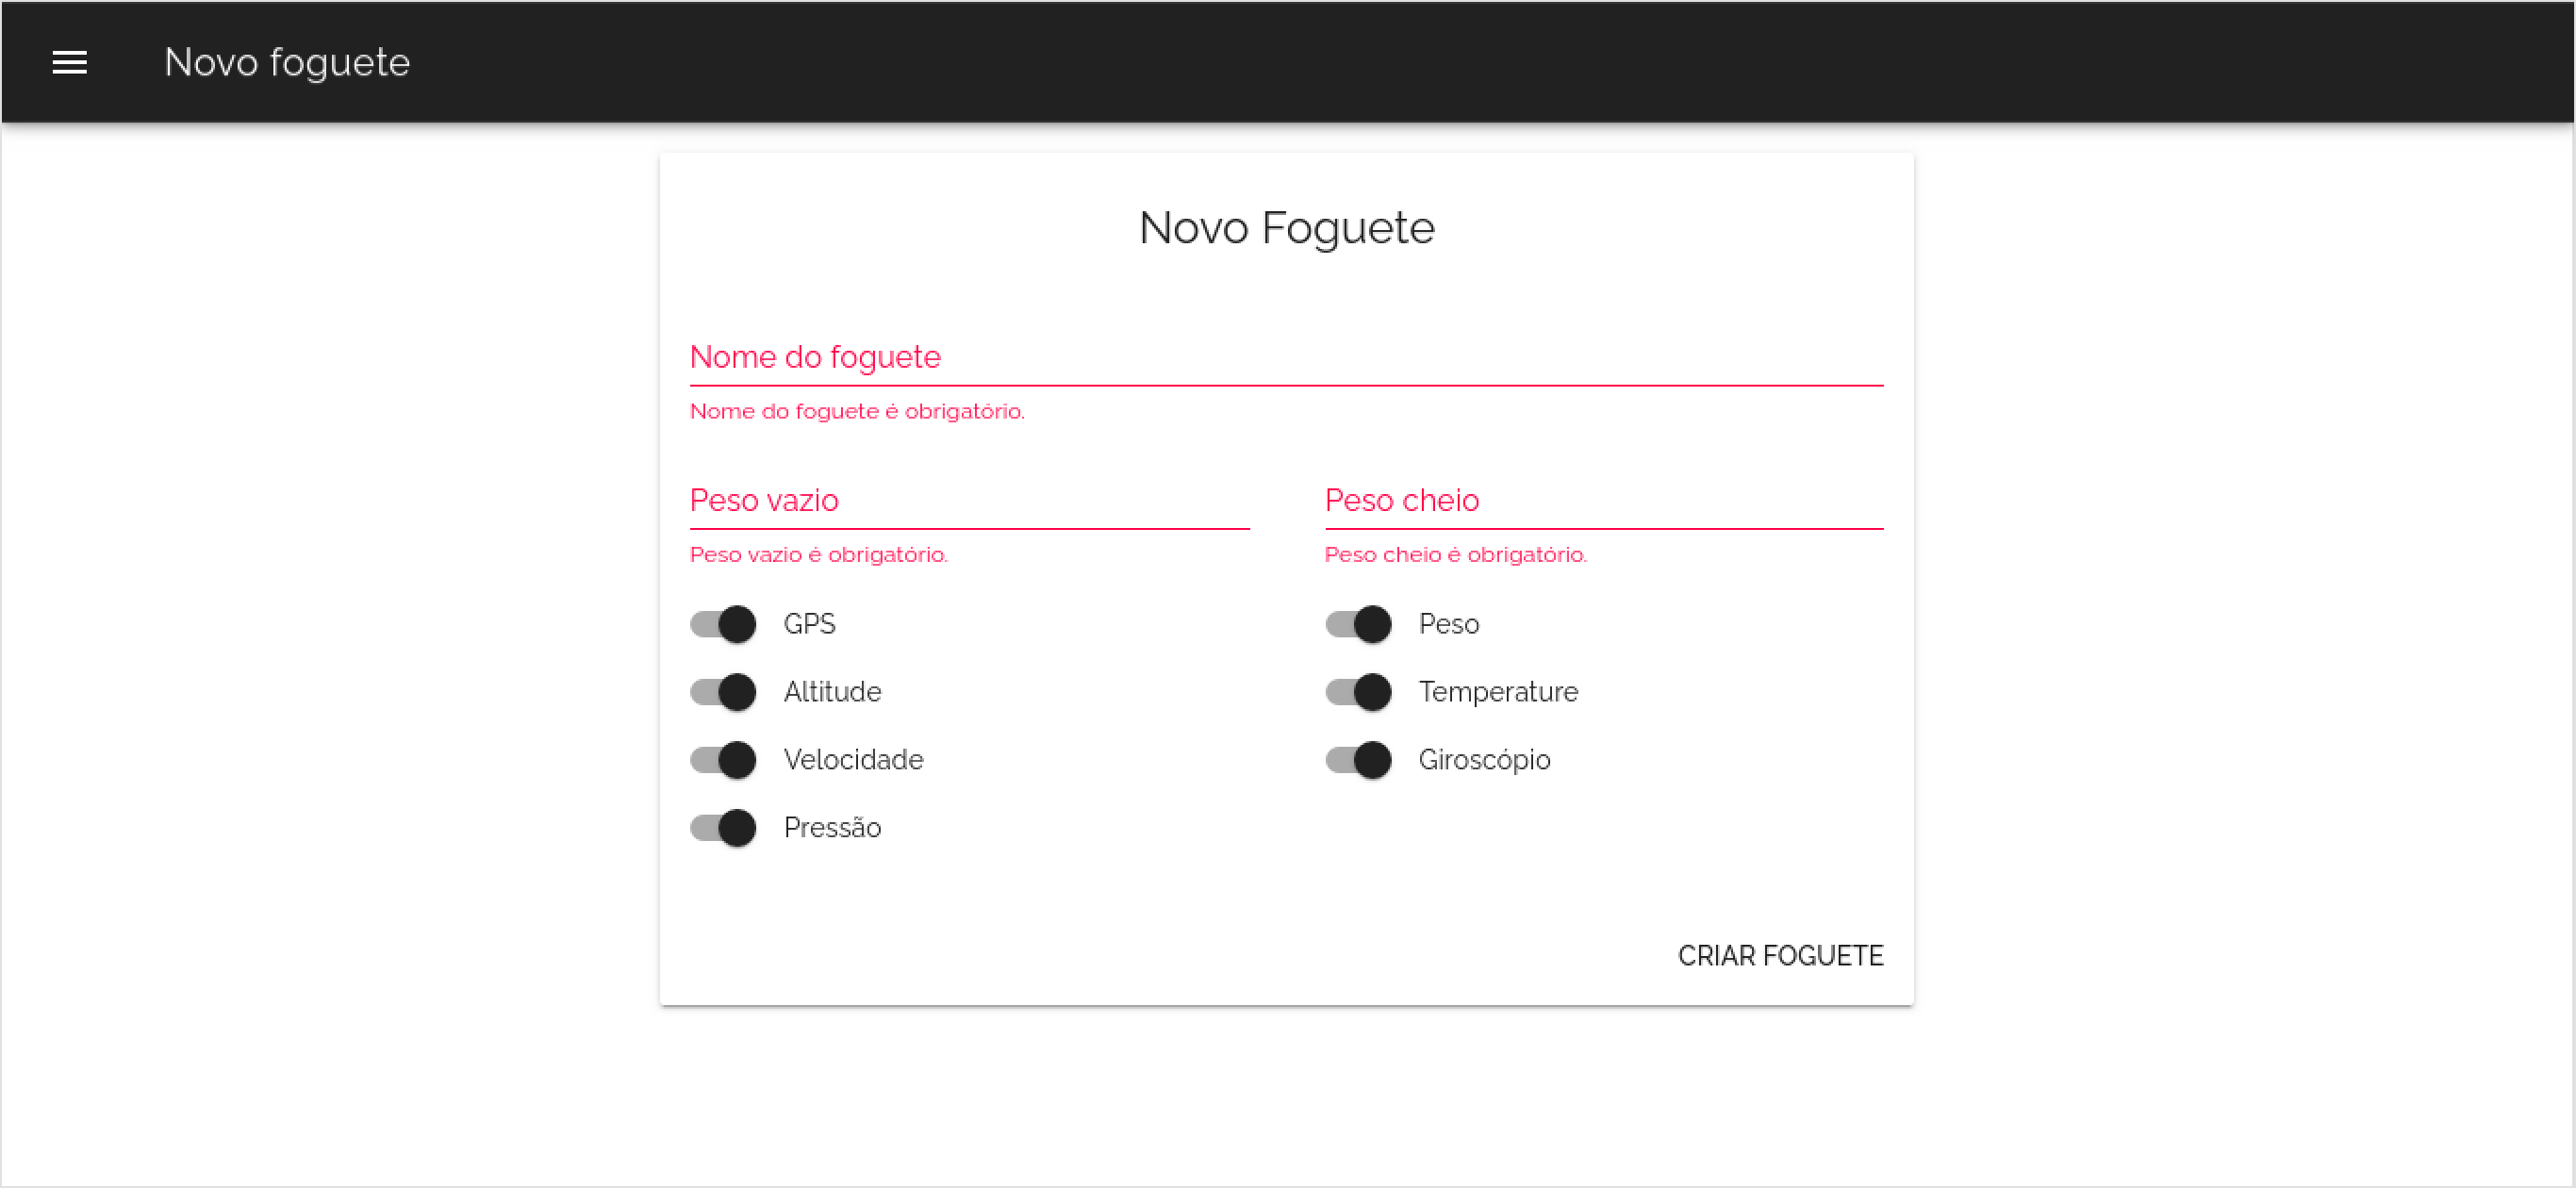
\includegraphics[keepaspectratio=true,scale=0.33]{figuras/telas_software/1-error.png}
	\caption{Tela de criação de foguete com erros demonstrando as validações feitas.}
	\label{fig:cria_foguete_error}
\end{figure}

\subsection{Criação de Hardware e Comandos}

Uma das principais funcionalidade do projeto, é permitir que o software seja utilizado em diferentes hardwares, caso seja compatível com as especificações técnicas. Portanto, a Figura \ref{fig:cria_hardware} permite que os usuários informe qual o nome hardware está sendo usado, o Baudrate e a porta serial para a comunicação.

\begin{figure}[h!]
	\centering
		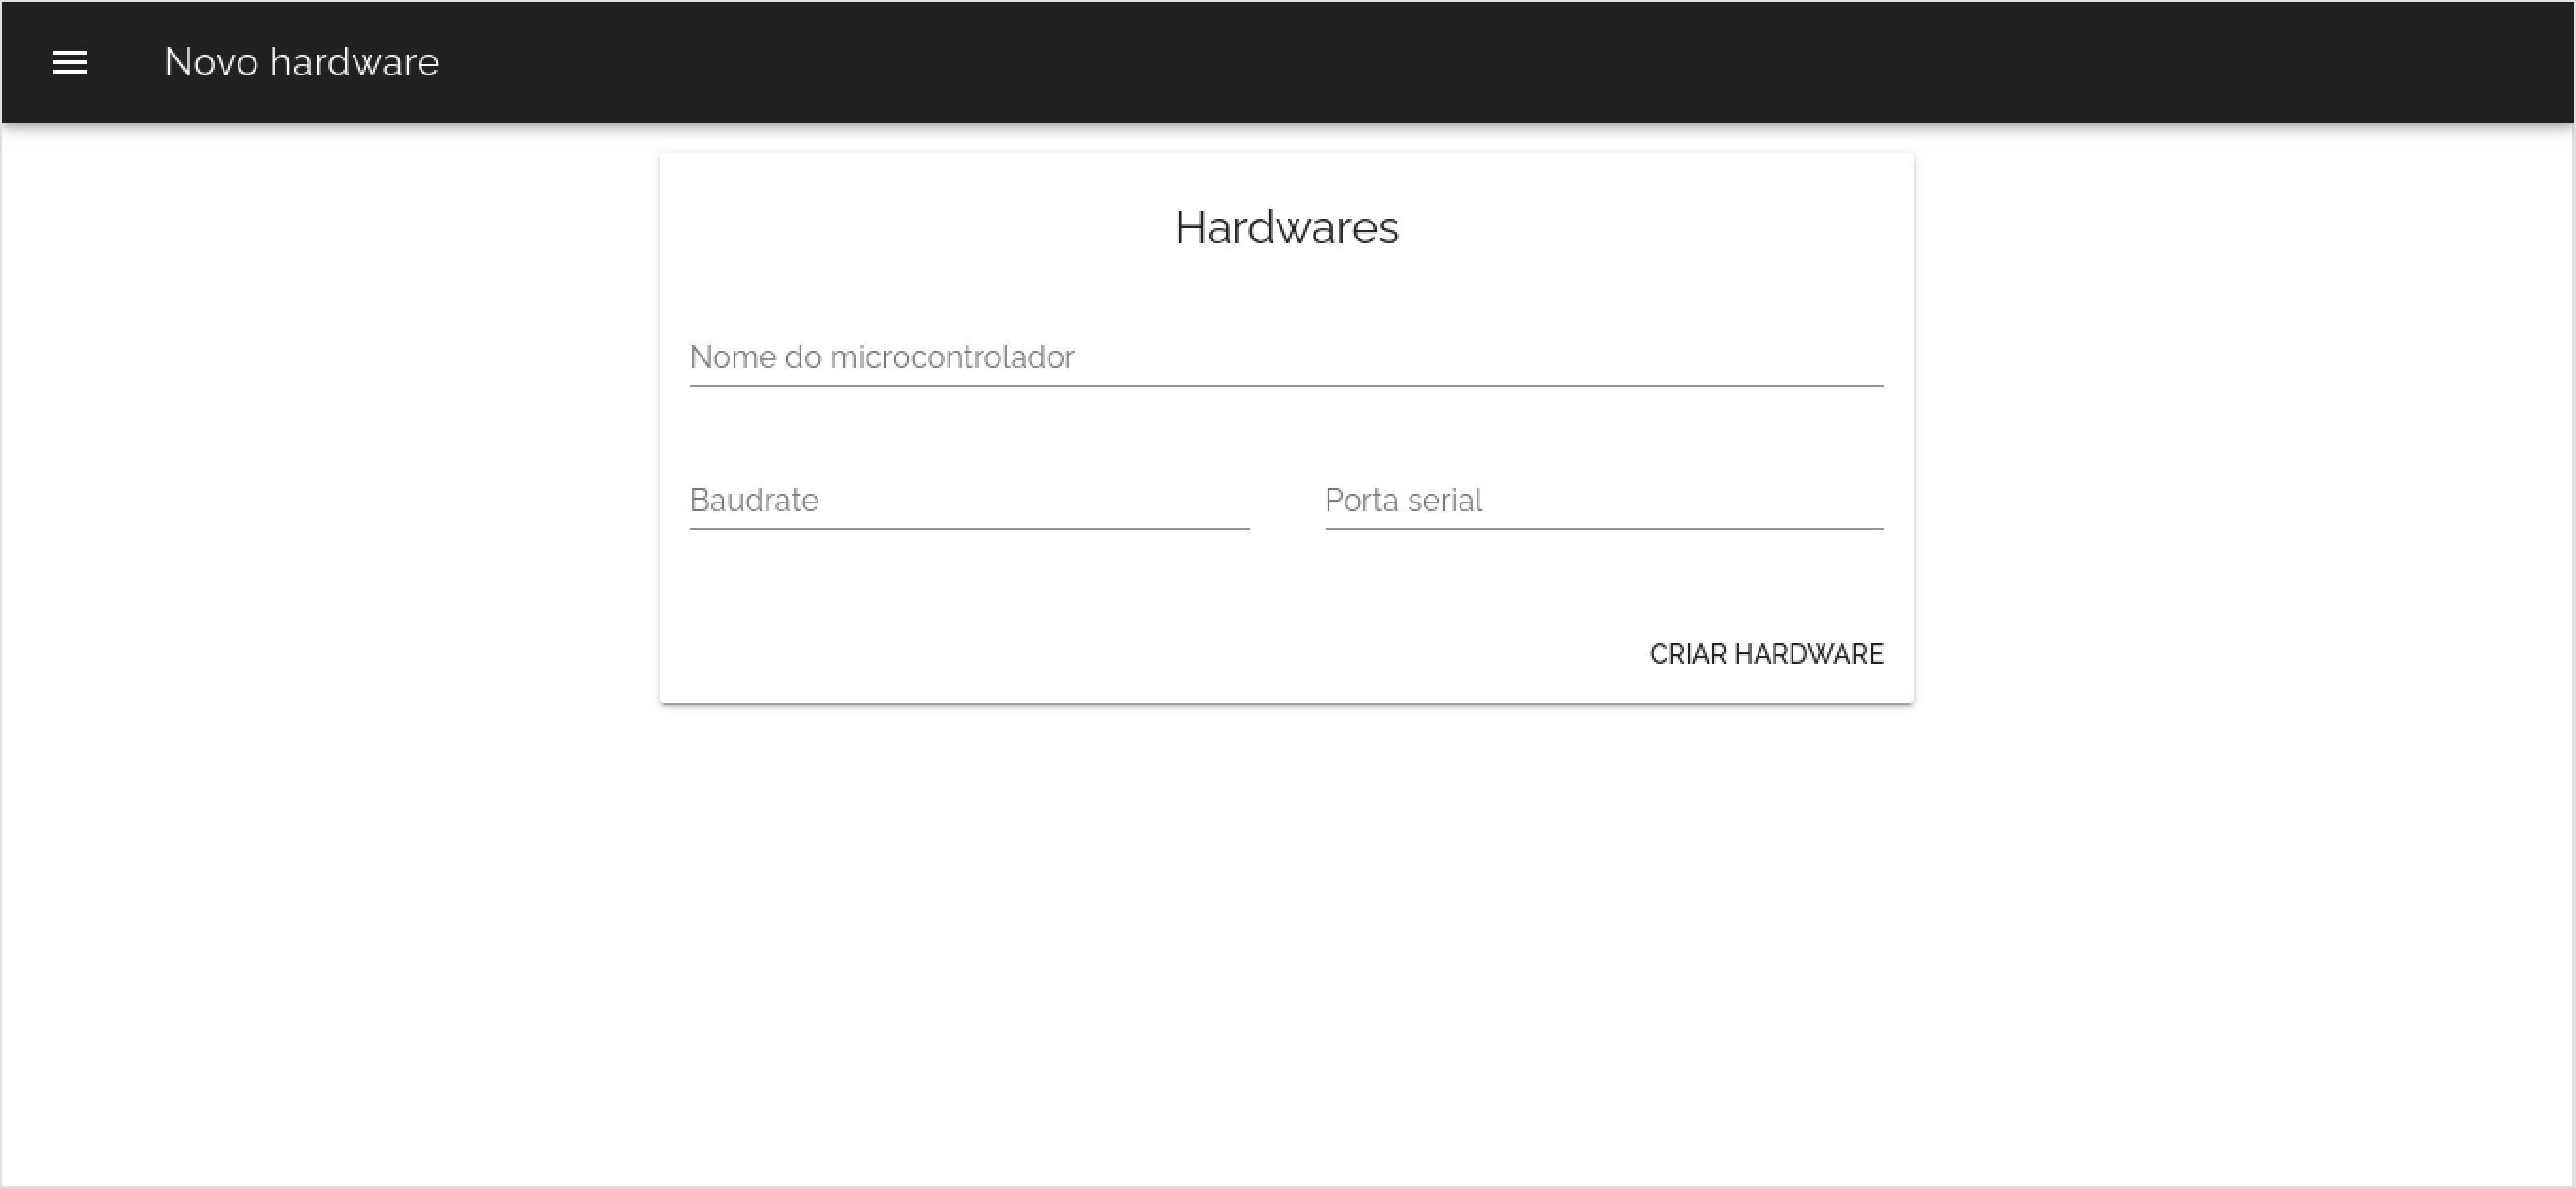
\includegraphics[keepaspectratio=true,scale=0.33]{figuras/telas_software/2.png}
	\caption{Tela de criação de hardware}
	\label{fig:cria_hardware}
\end{figure}

Para garantir o bom funcionamento do sistema, todas essas informações são importantes, portanto foi feito a validação para impedir que o usuário esqueça de inserir alguma informação obrigatória, como apresentado na Figura \ref{fig:cria_hardware_error}.

\begin{figure}[h!]
	\centering
		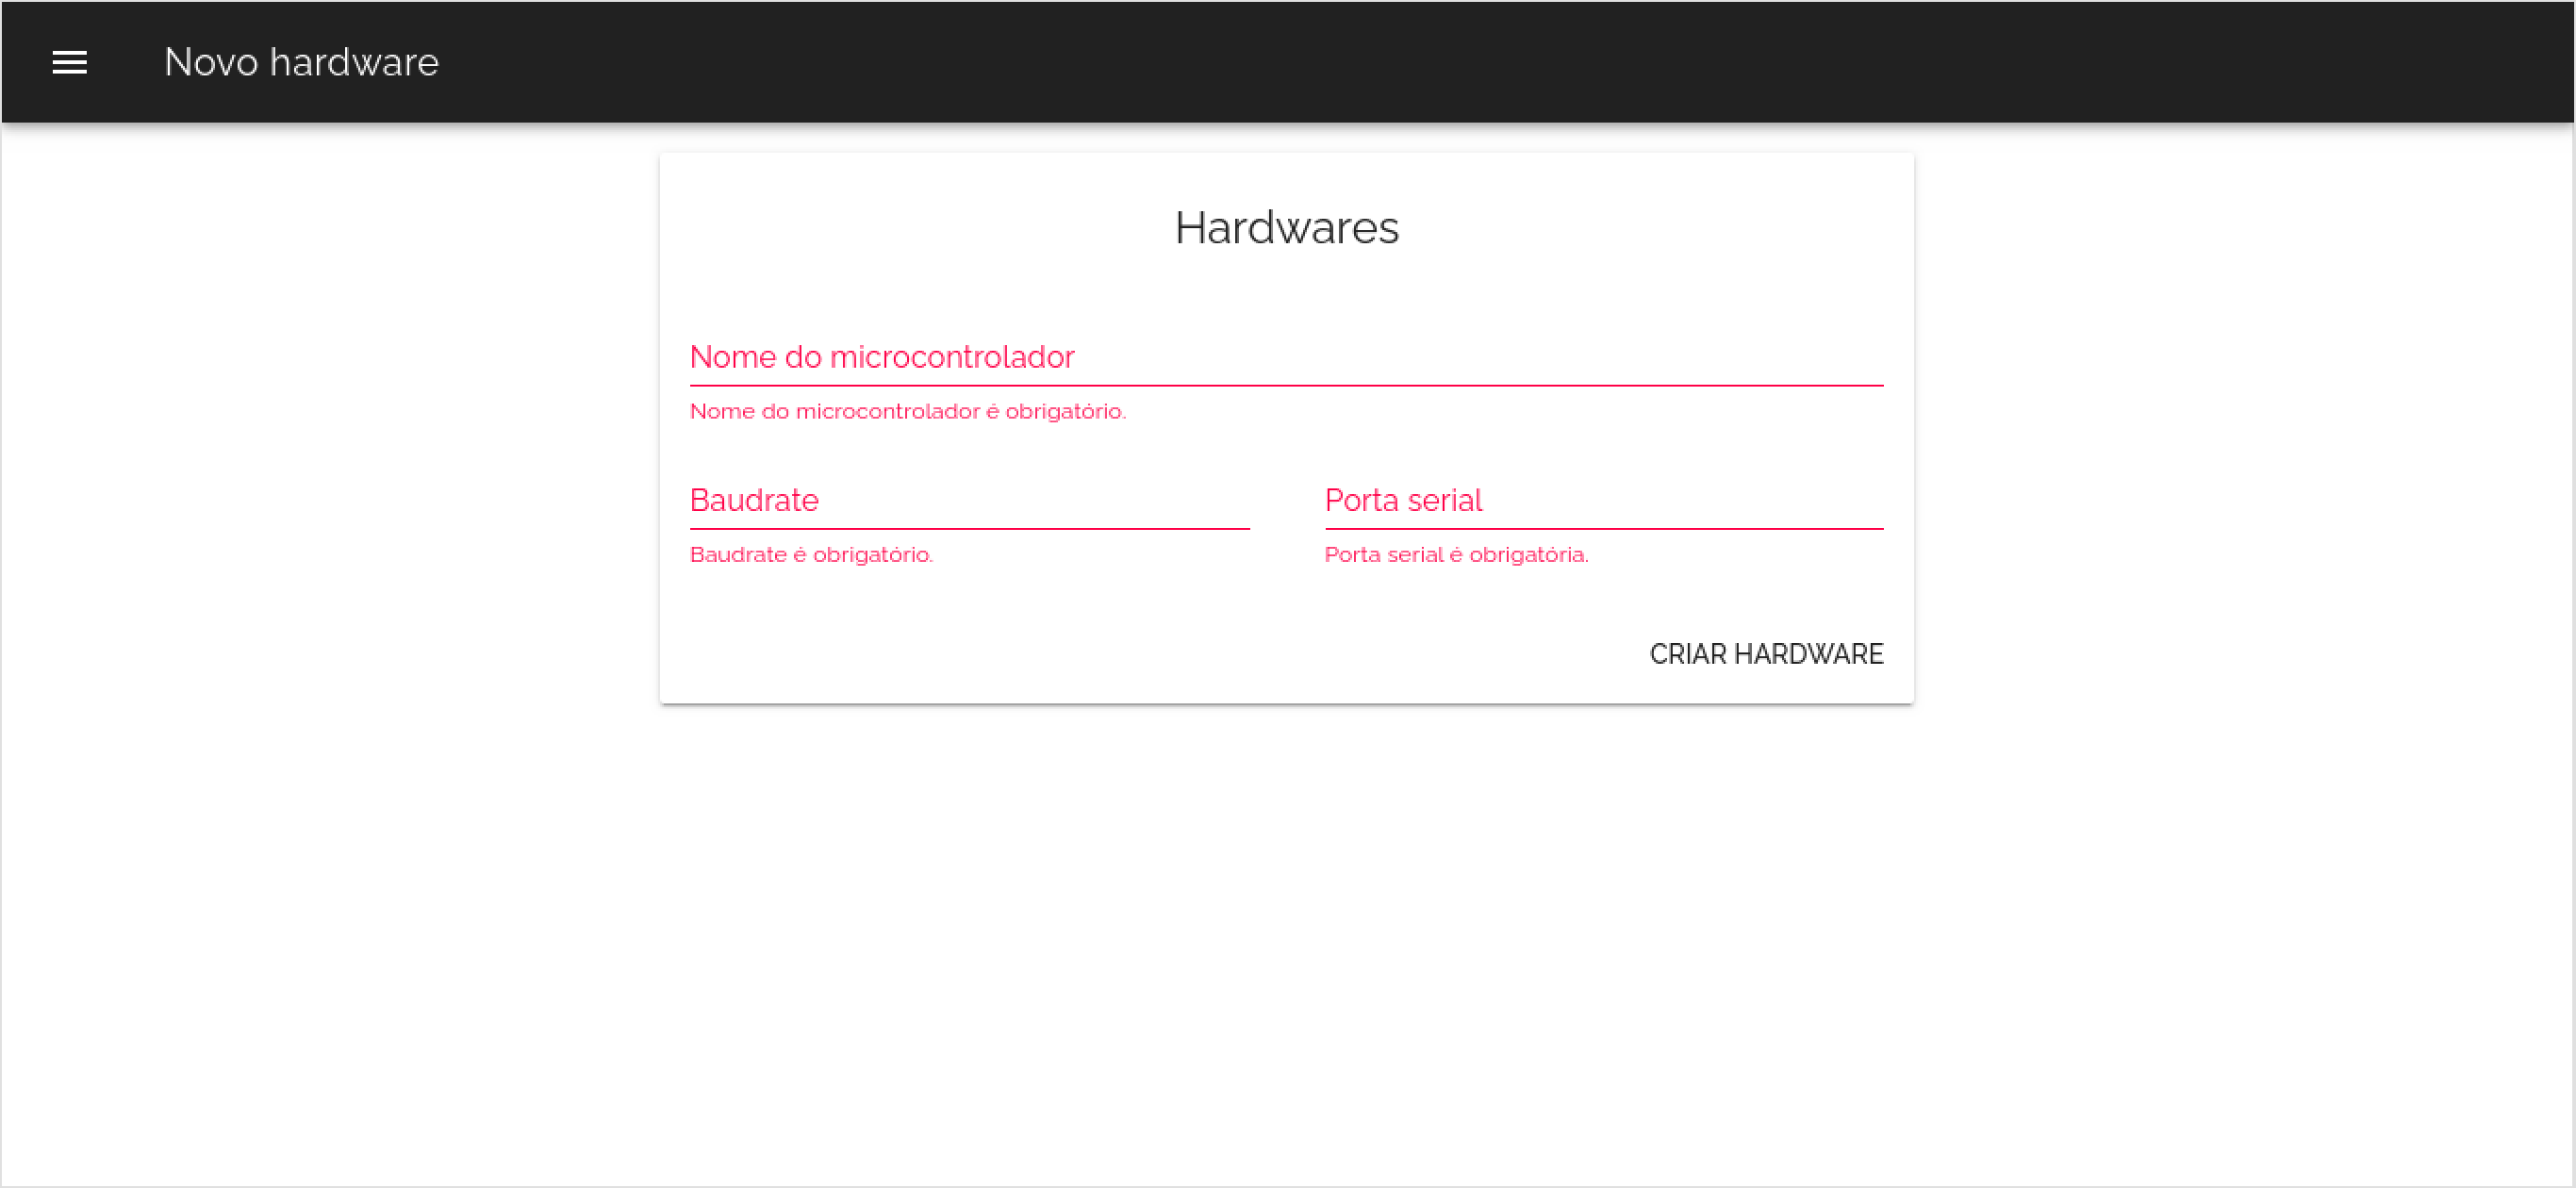
\includegraphics[keepaspectratio=true,scale=0.33]{figuras/telas_software/2-error.png}
	\caption{Tela de criação de hardware com erros demonstrando as validações feitas.}
	\label{fig:cria_hardware_error}
\end{figure}

Ao cadastrar o Hardware a ser usado, é necessário informar também quais comandos esse hardware está apto a receber, como apresentado na Figura \ref{fig:cria_comandos_hardware}. portanto, os usuários e clientes da Capital poderão inserir quais comandos serão enviados ao hardware
\begin{figure}[h!]
	\centering
		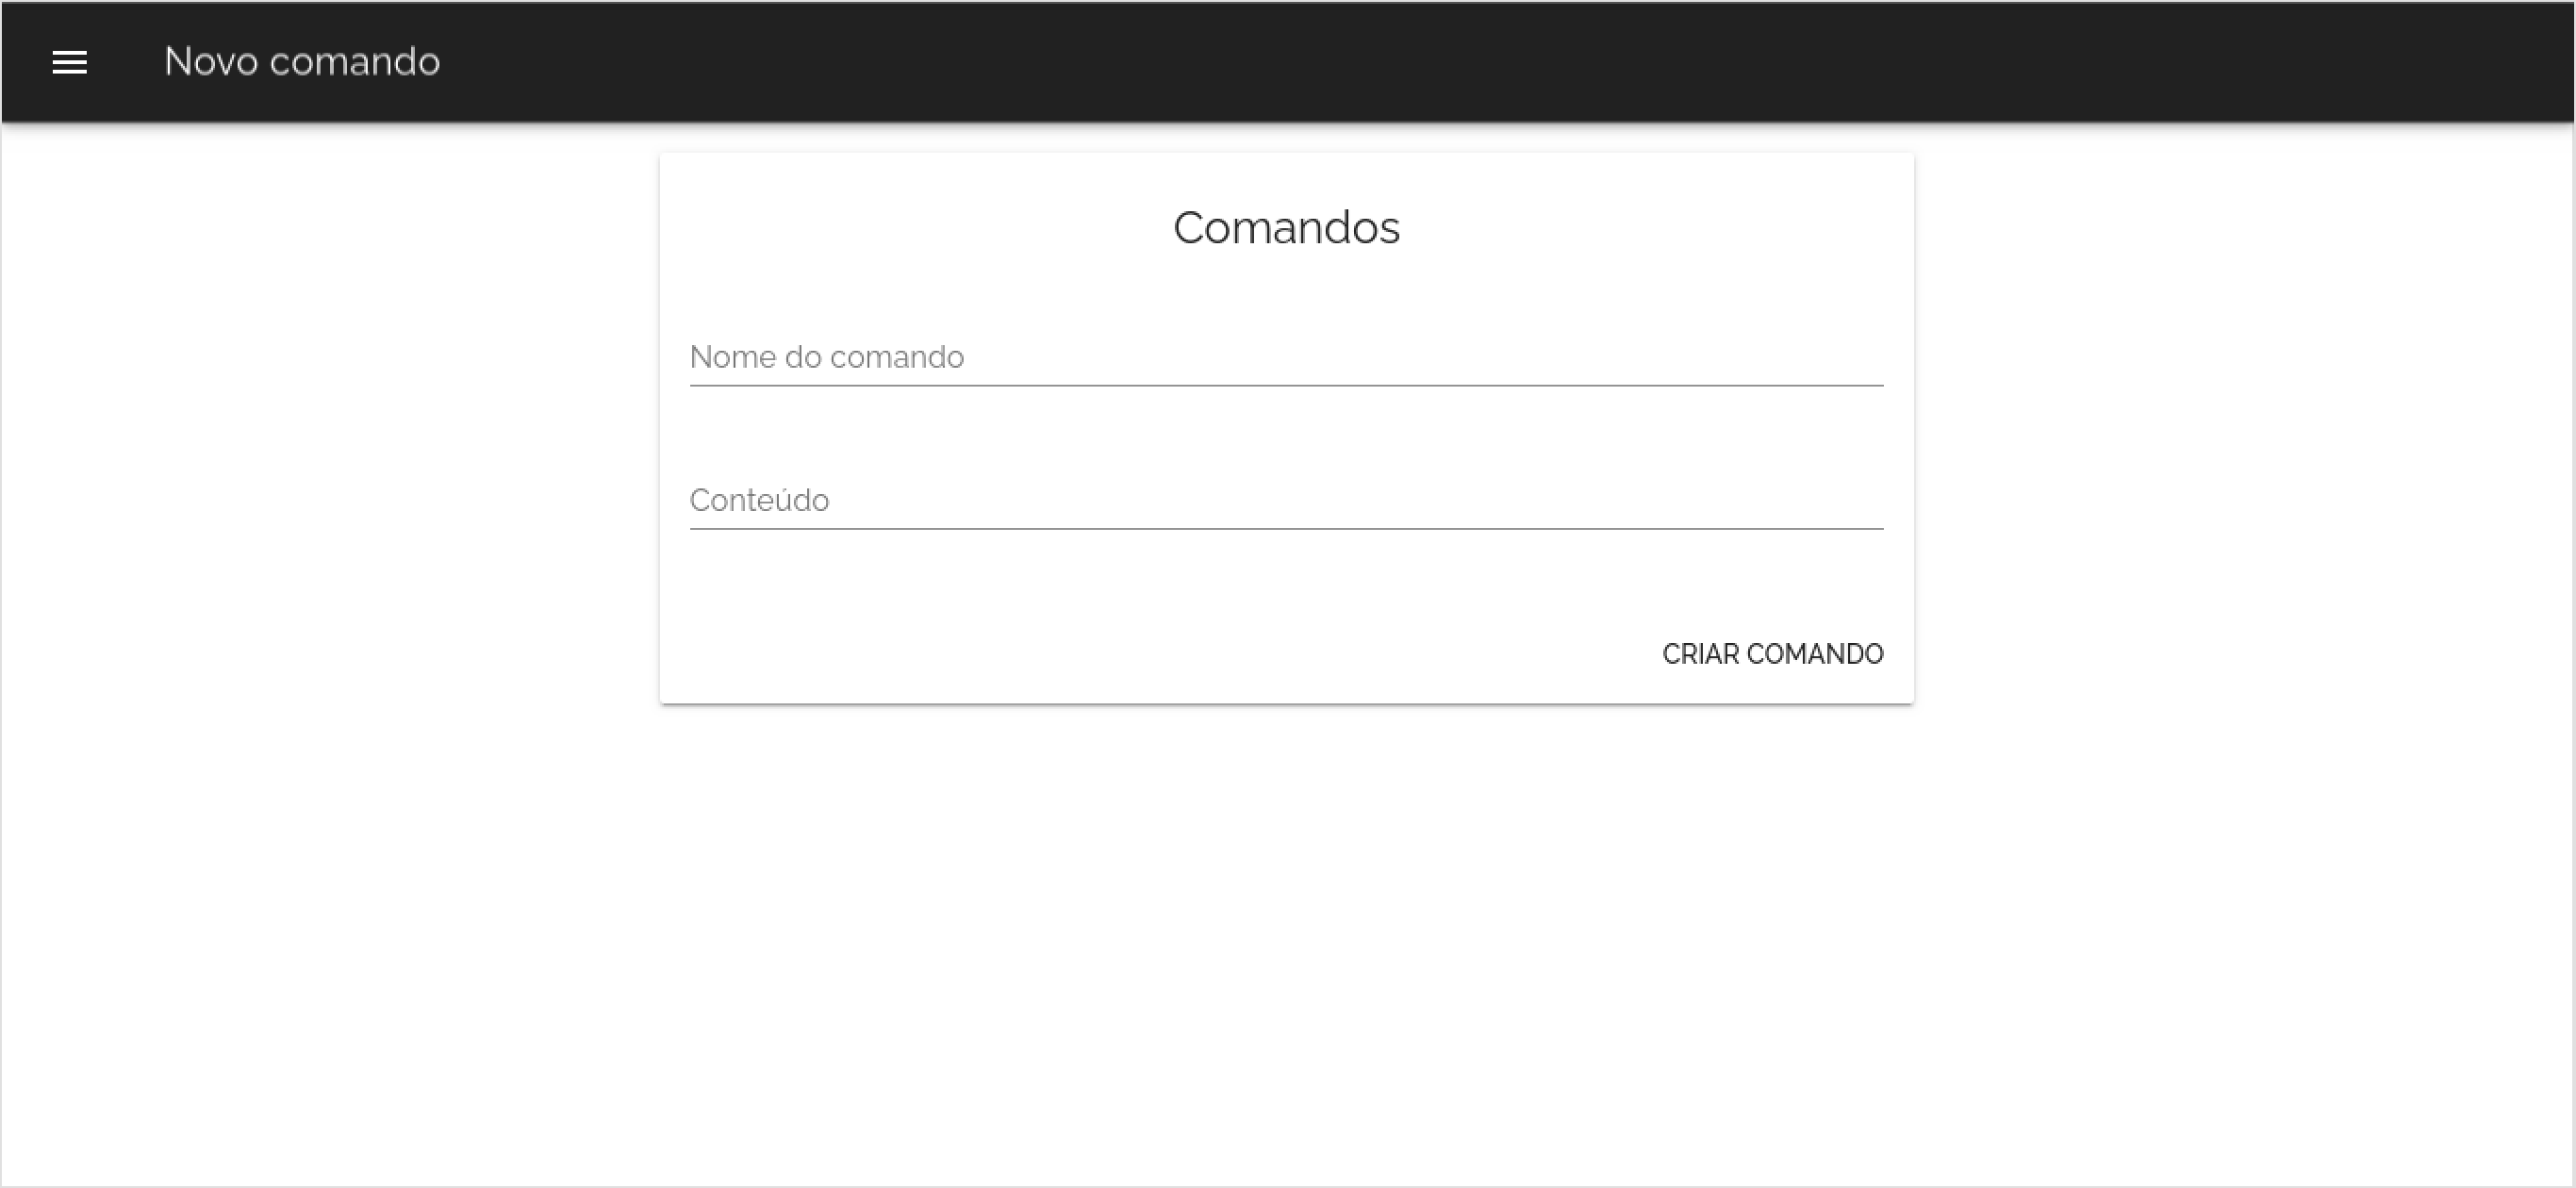
\includegraphics[keepaspectratio=true,scale=0.33]{figuras/telas_software/3.png}
	\caption{Tela de criação de comando para o hardware.}
	\label{fig:cria_comandos_hardware}
\end{figure}

\subsection{Ciclo de missão}

\begin{figure}[h!]
	\centering
		
\includegraphics[keepaspectratio=true,scale=0.33]{figuras/telas_software/4.png}
	\caption{Tela de inicio de missão.}
	\label{fig:inicia_missao}
\end{figure}

Após cadastrar o foguete e o hardware que está sendo usado pode se iniciar o ciclo da missão, iniciando na tela apresentada na Figura \ref{fig:inicia_missao}.

Após confirmar a intenção de iniciar uma missão, é solicitado ao usuário o cadastro da missão informando nome e apogeu esperado (Figura \ref{fig:dados_missao}) e seleciona o foguete como apresentado na Figura \ref{fig:escolhe_foguete}.
\begin{figure}[h!]
	\centering
		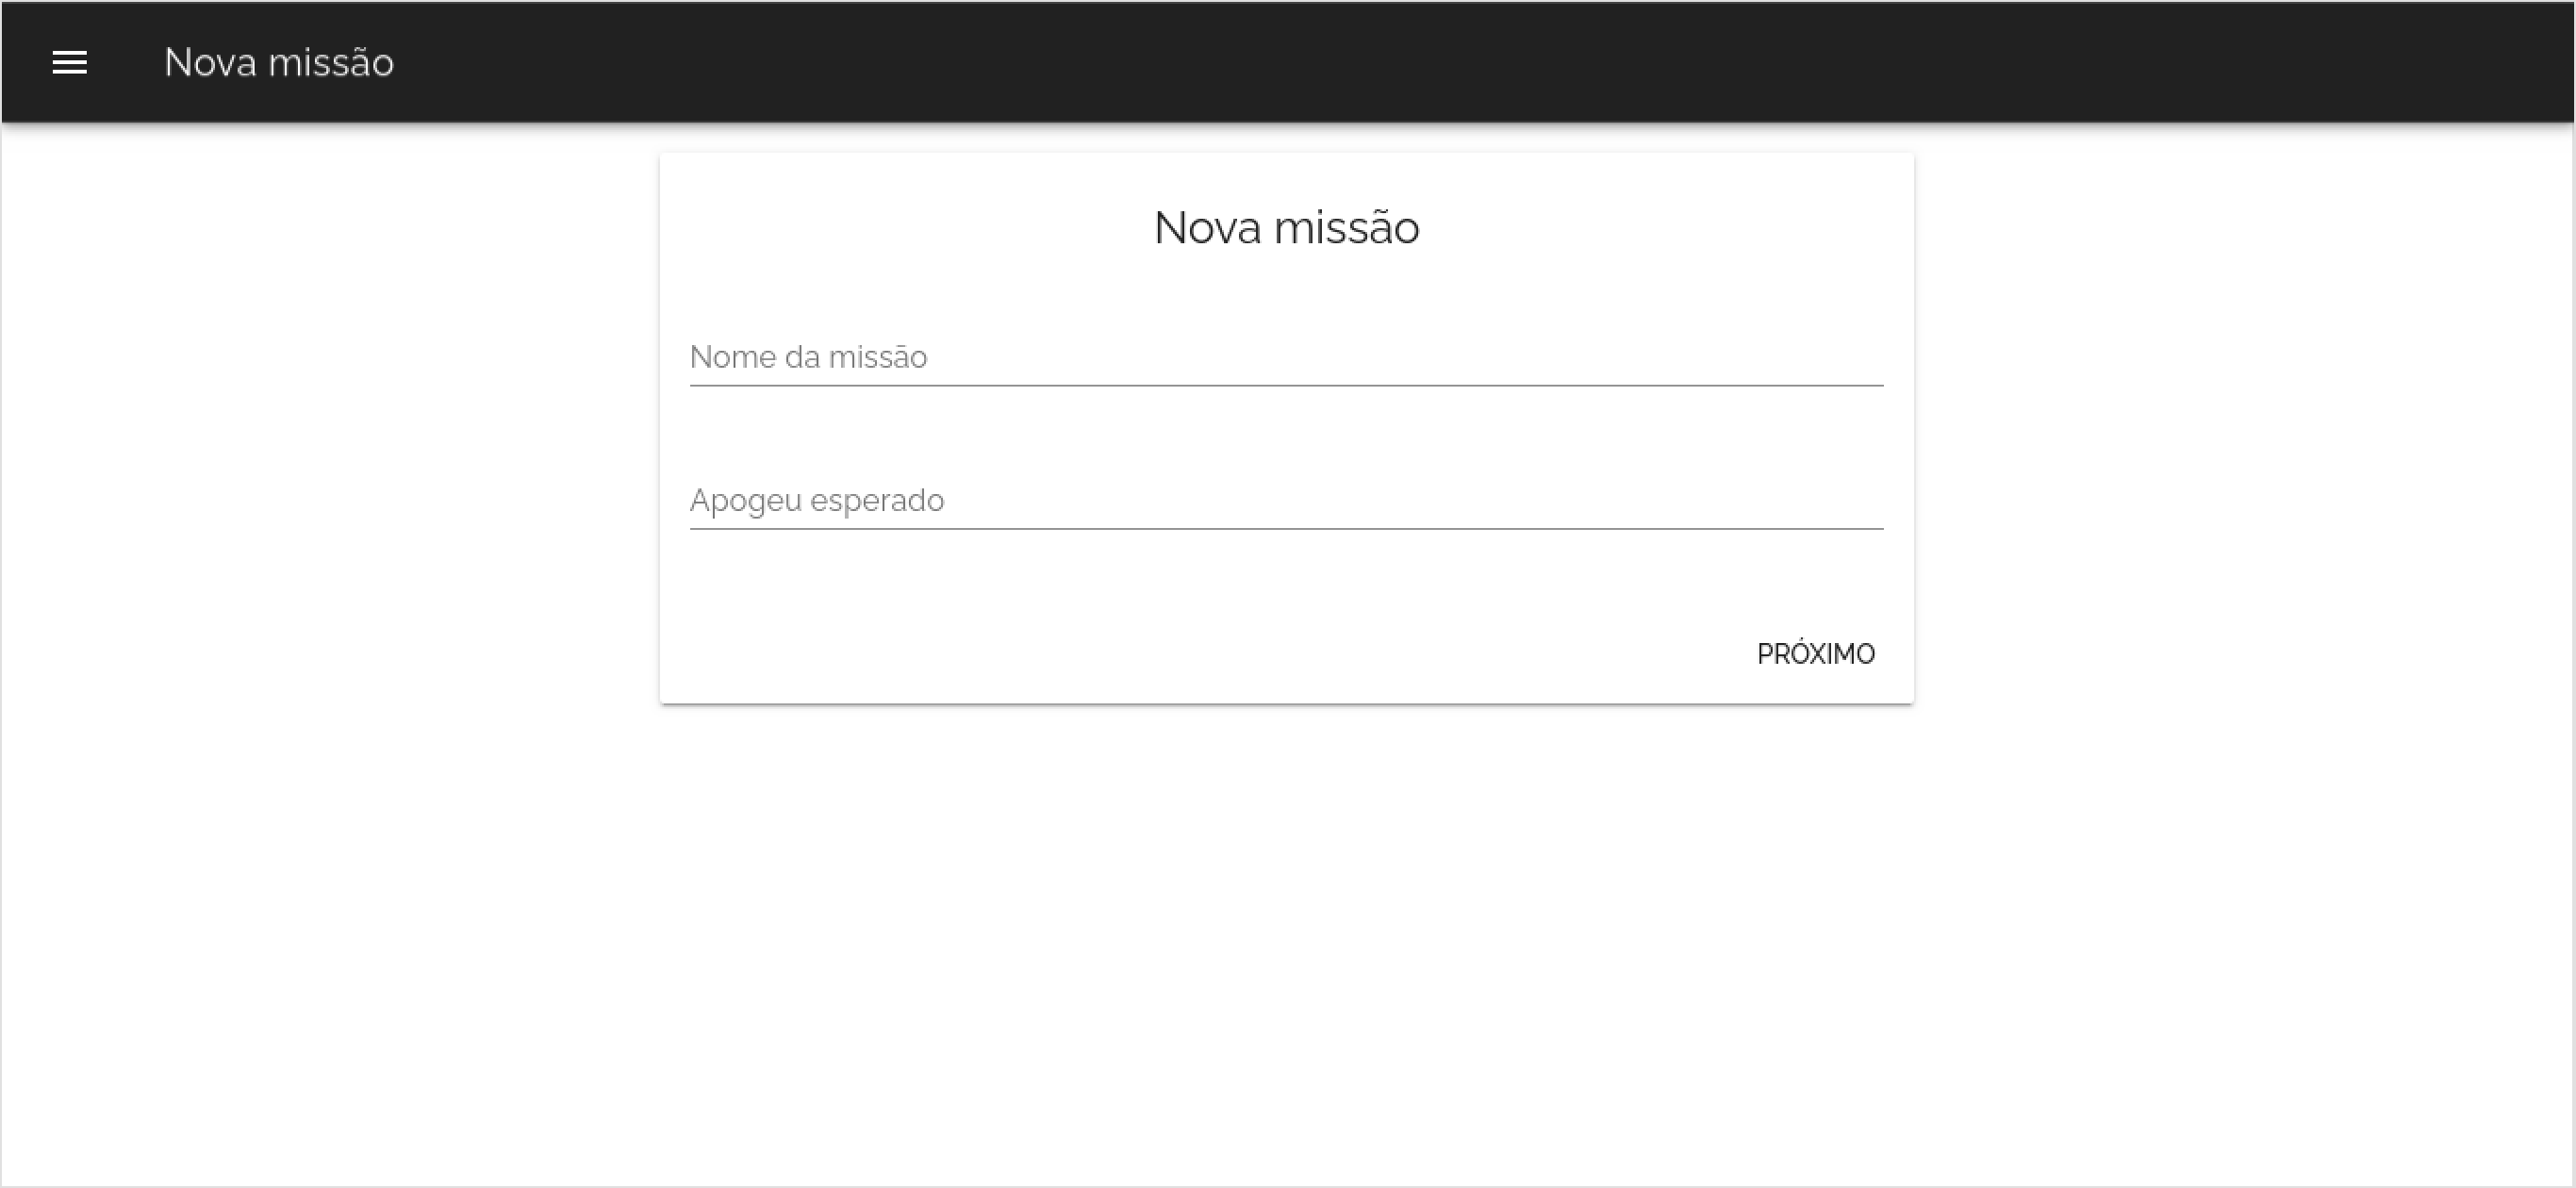
\includegraphics[keepaspectratio=true,scale=0.33]{figuras/telas_software/5.png}
	\caption{Tela para inserção dos dados de uma nova missão.}
	\label{fig:dados_missao}
\end{figure}

\begin{figure}[h!]
	\centering
		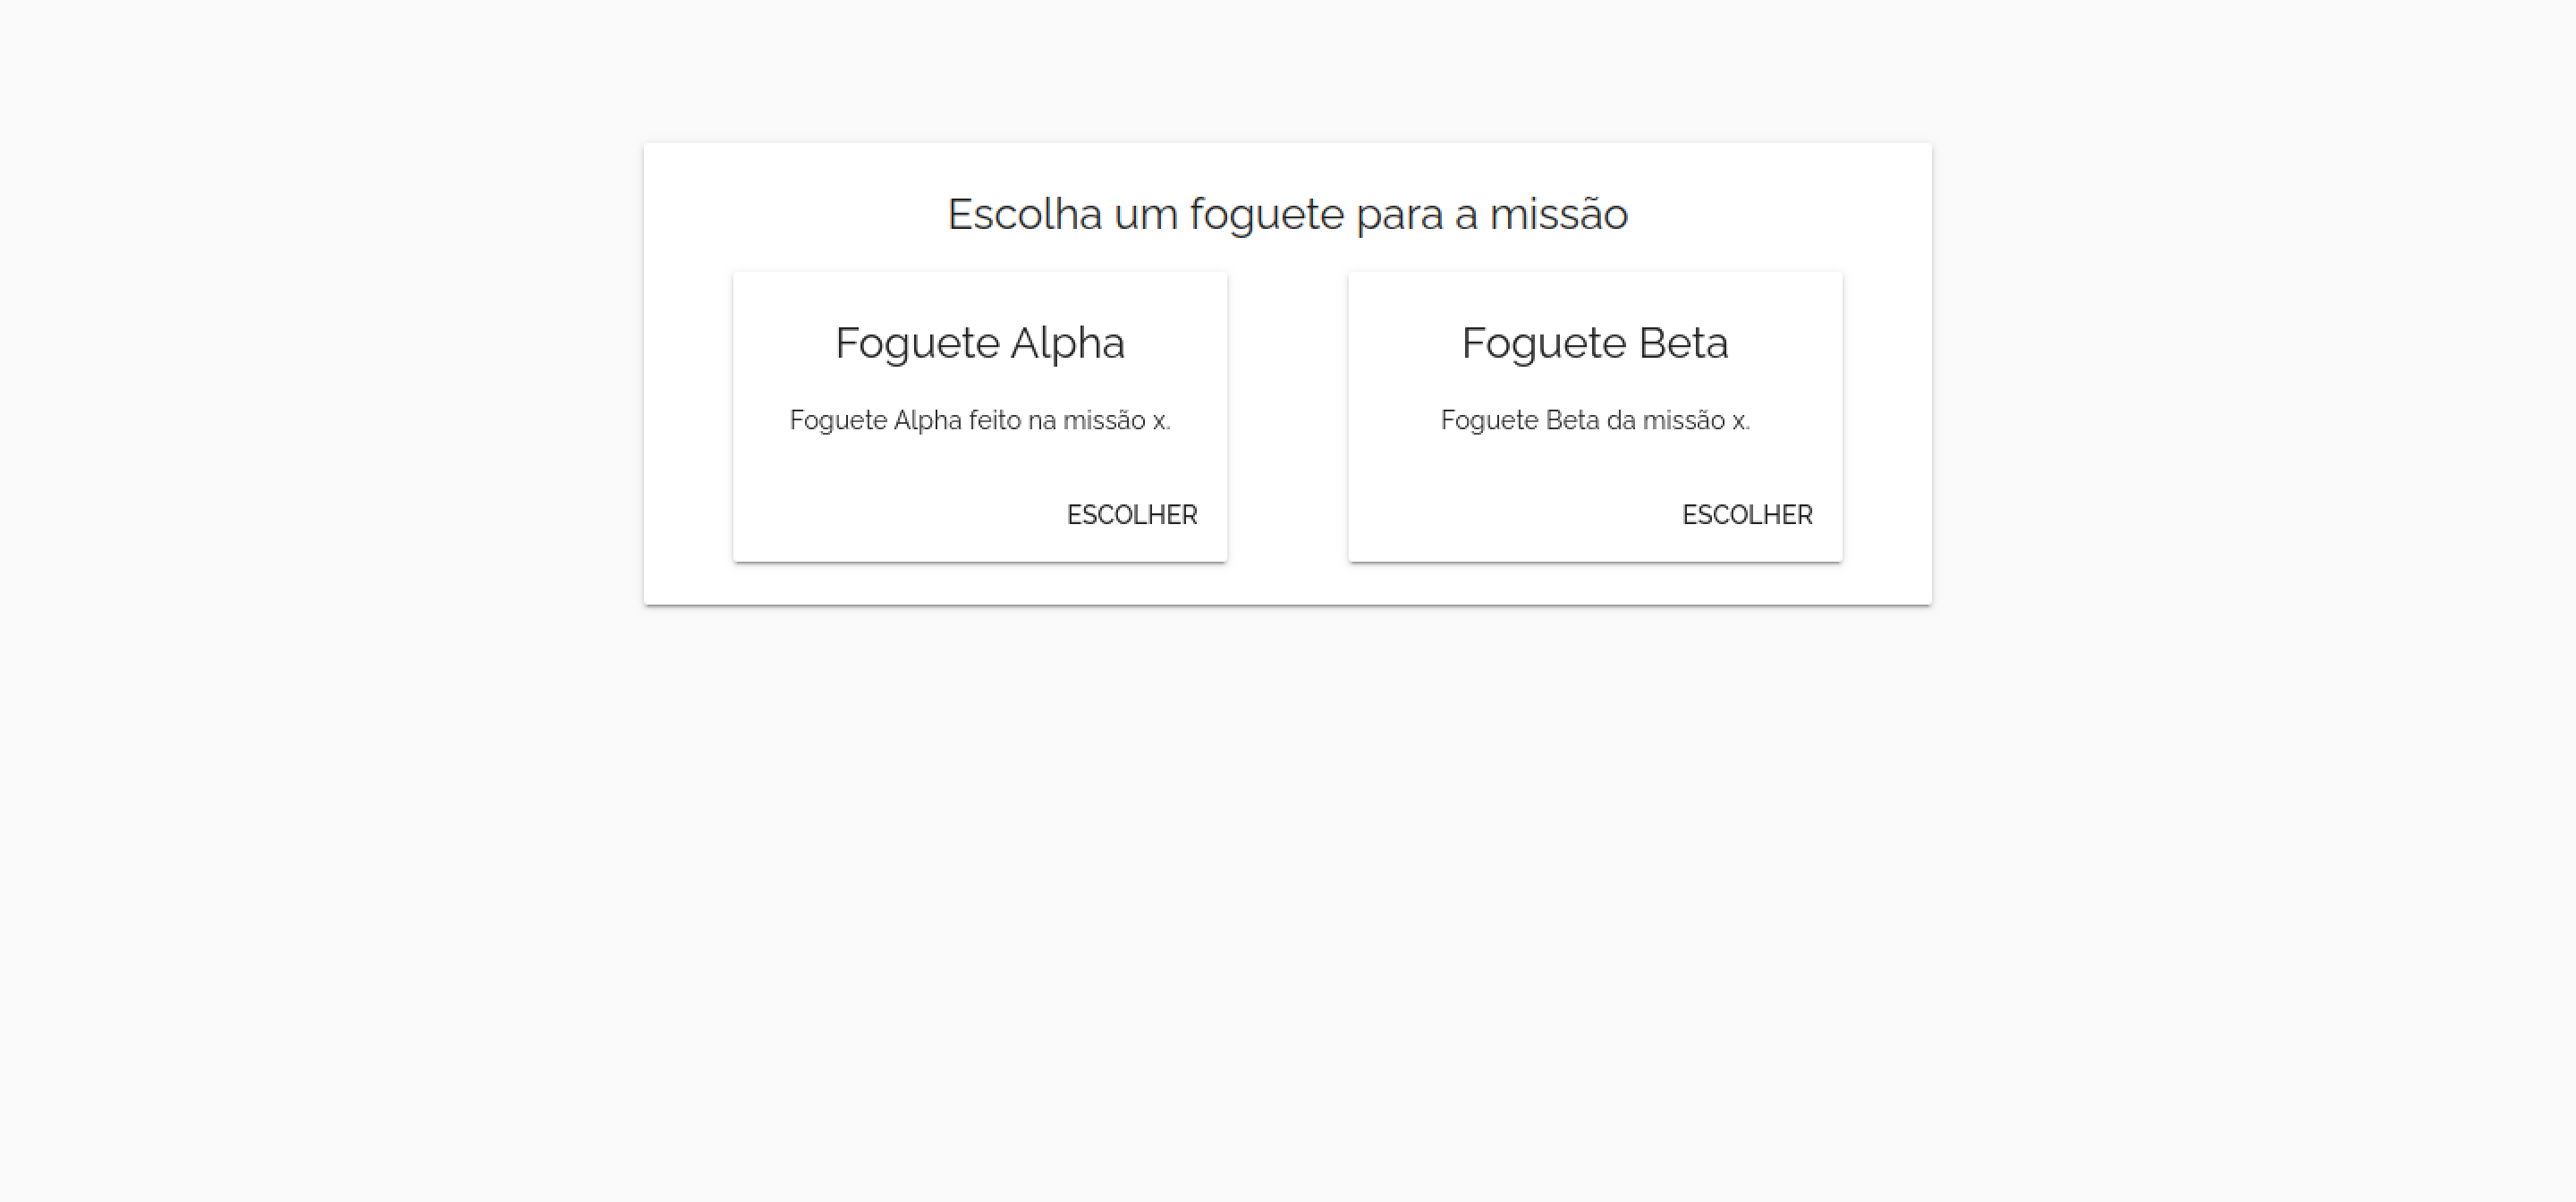
\includegraphics[keepaspectratio=true,scale=0.33]{figuras/telas_software/6.png}
	\caption{Tela de escolha do foguete para a missão.}
	\label{fig:escolhe_foguete}
\end{figure}

Após todo processo de criação de uma missão, o usuário poderá acompanhar o todas as etapas da missão, começando pela etapa de abastecimento, conforme apresentado na Figura \ref{fig:inicio_ignicao}.

\begin{figure}[h!]
	\centering
		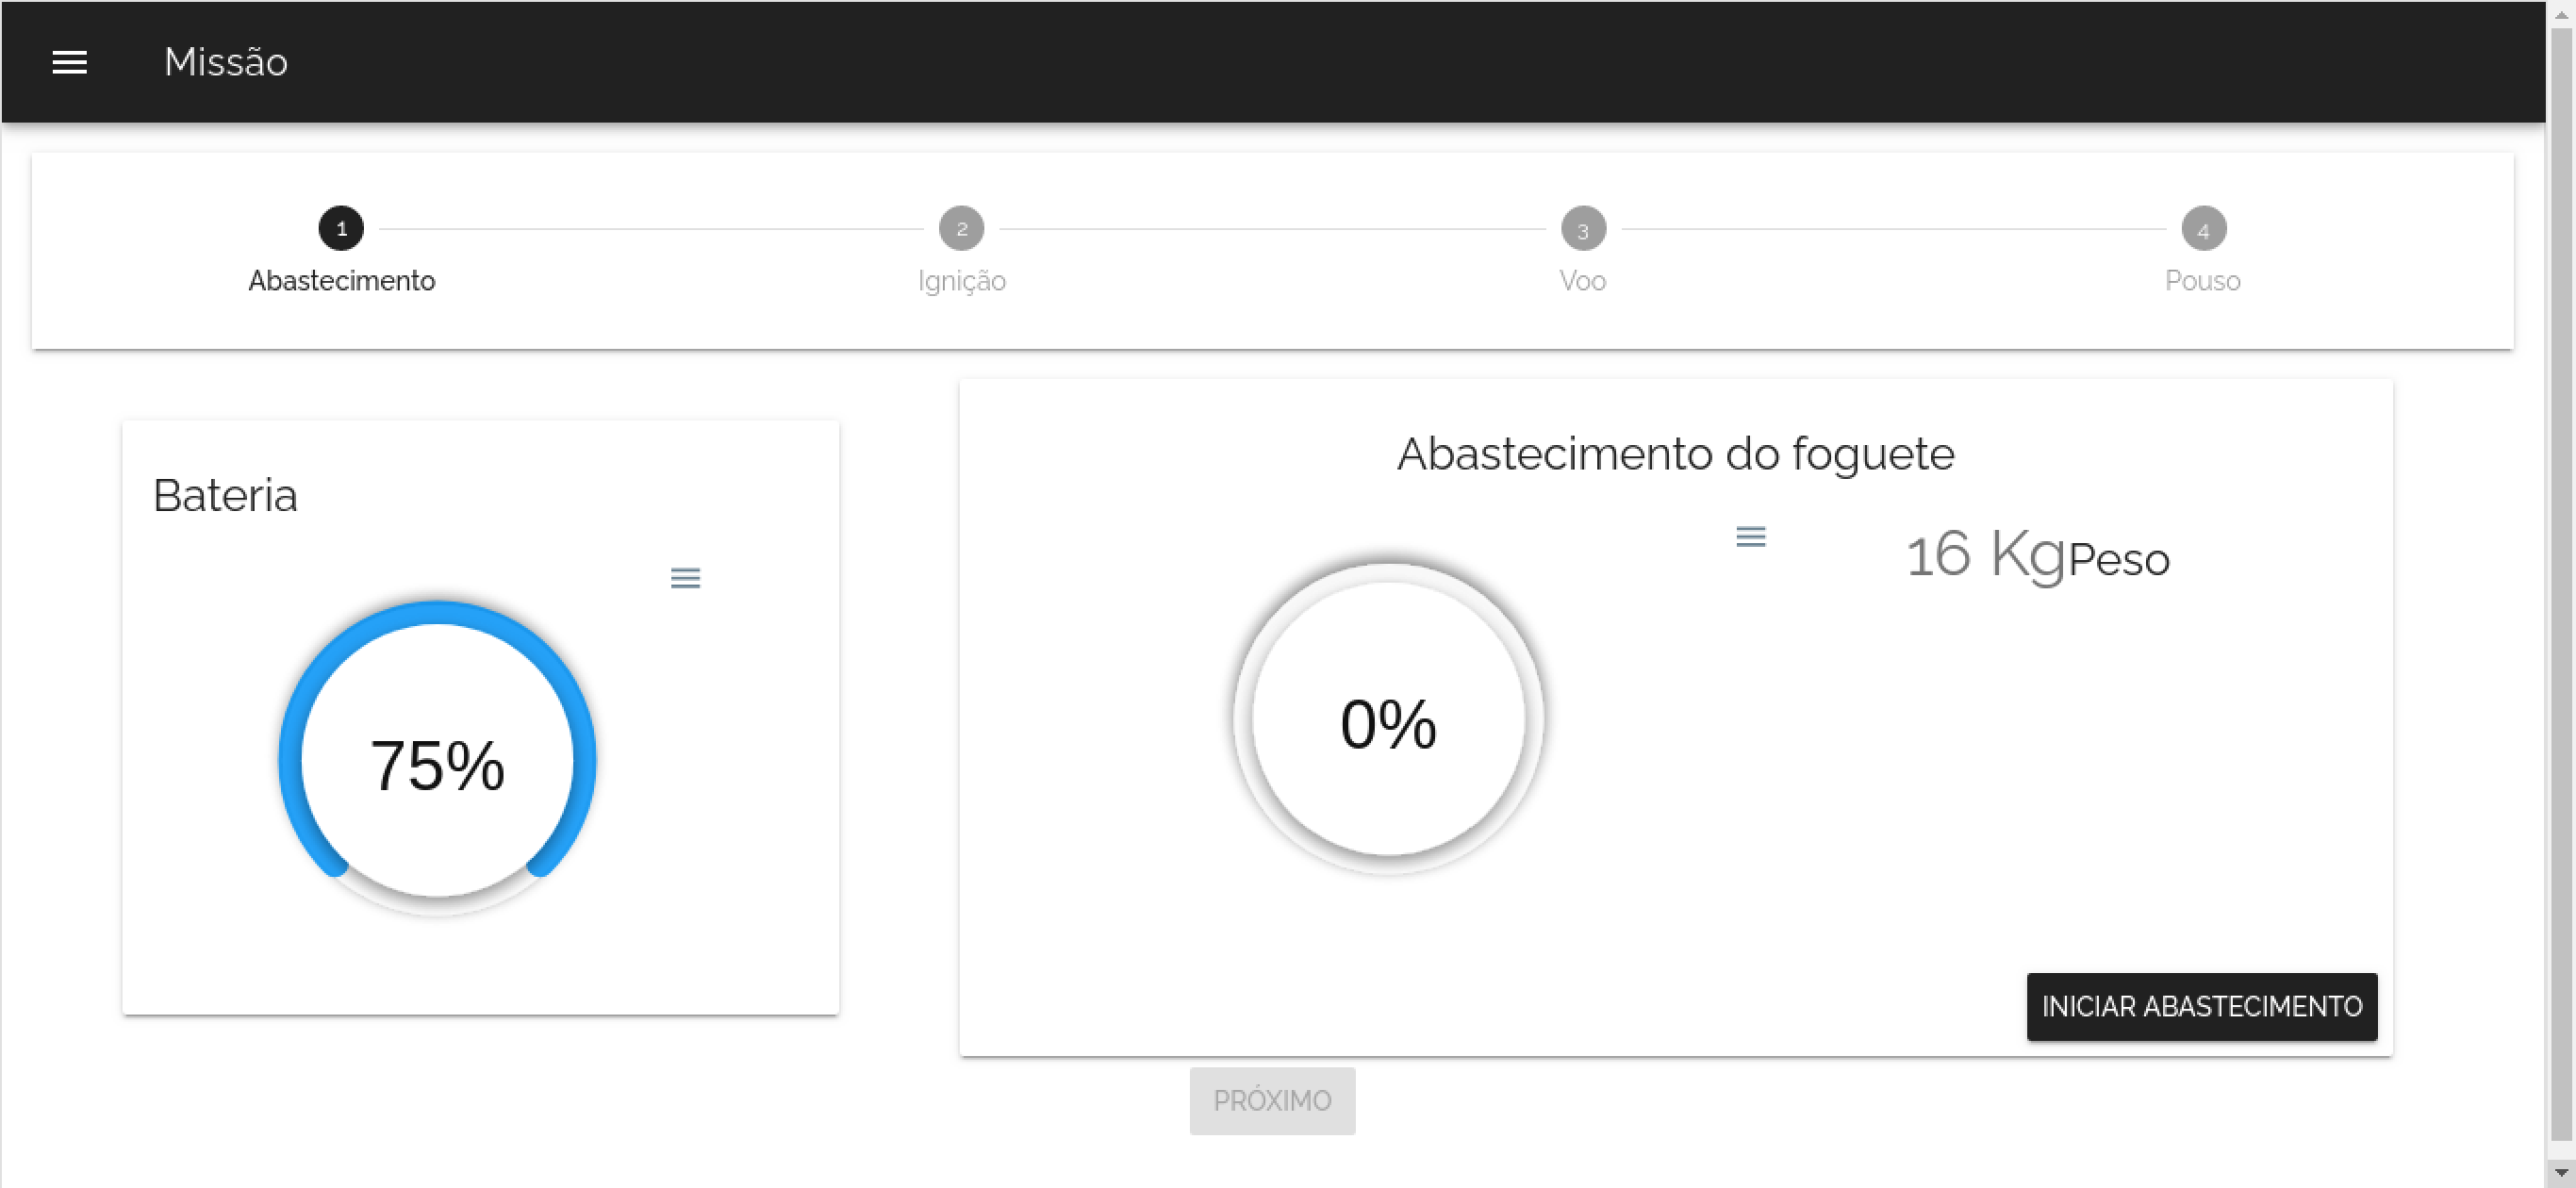
\includegraphics[keepaspectratio=true,scale=0.33]{figuras/telas_software/7.png}
	\caption{Tela inicial da missão, com os dados de abastecimento.}
	\label{fig:inicio_ignicao}
\end{figure}

A Figura \ref{fig:fim_ignicao} mostra o processo de ignição completo, com a porcentagem chegando em 100\%. O botão de "Próximo" é habilitado para o usuário prosseguir para a próxima etapa da missão. Em ambos os gráficos utilizados é possível baixar o gráfico em SVG, PNG ou CSV.

\begin{figure}[h!]
	\centering
		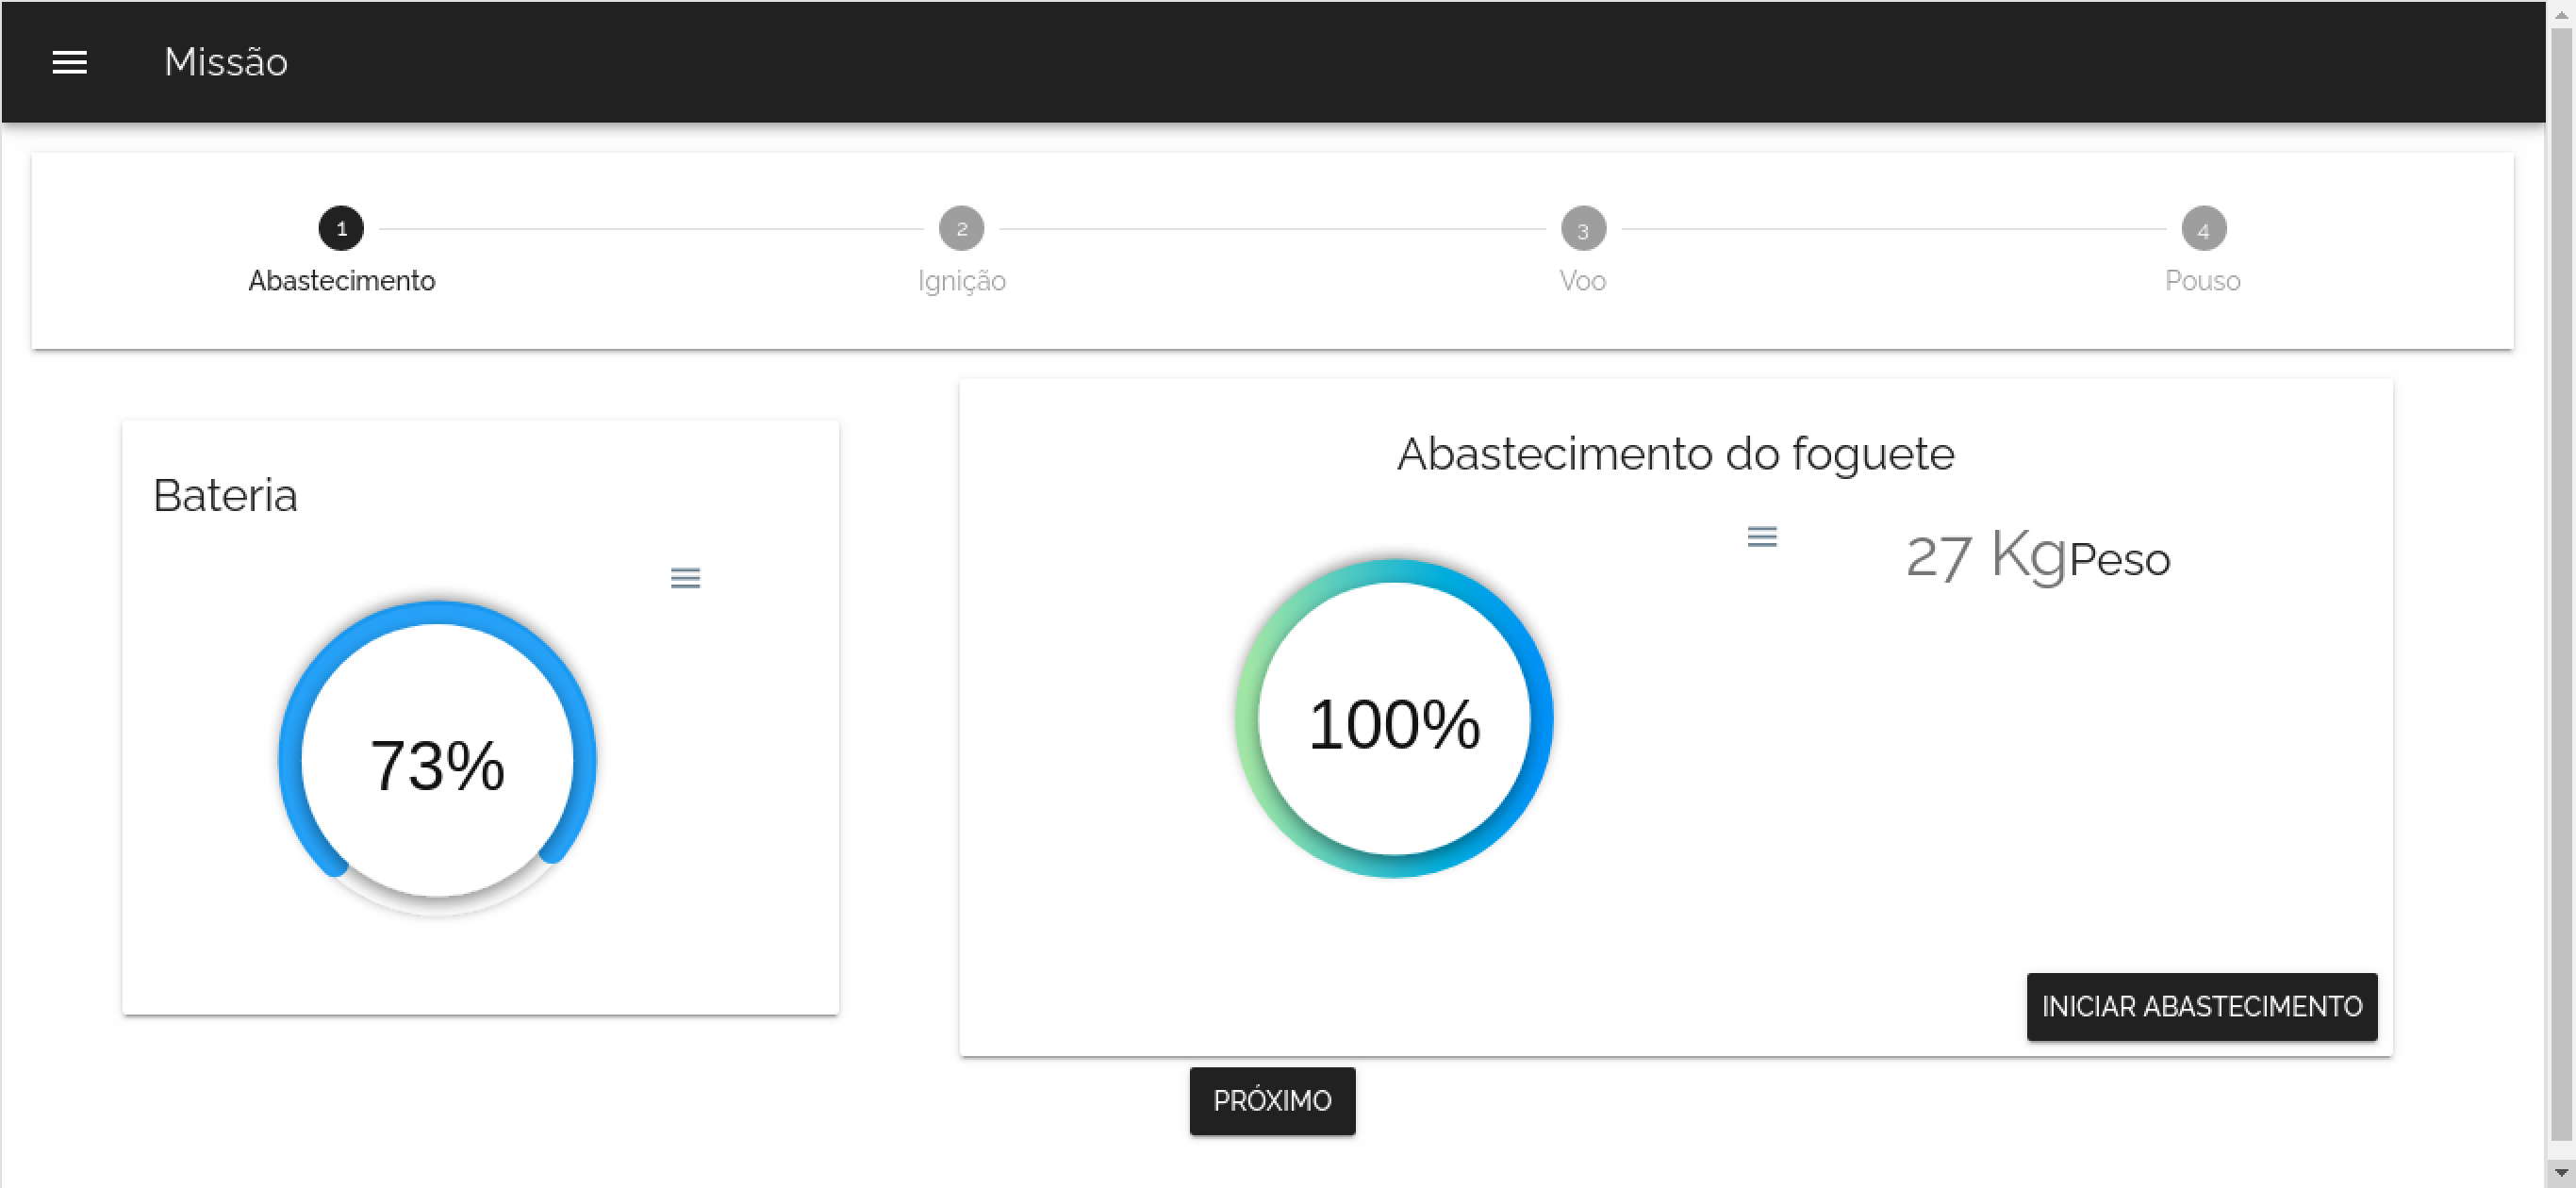
\includegraphics[keepaspectratio=true,scale=0.33]{figuras/telas_software/7-full.png}
	\caption{Tela da fase de abastecimento após o processo concluído.}
	\label{fig:fim_ignicao}
\end{figure}

\section{Construção Backend}

\subsection{API}

A API foi utilizada para desenvolver todos os serviços de consulta e alteração do banco de dados. No Apêndice \ref{documentacao_api} está documentado todos os \textit{endpoints} da API e seus respectivos métodos http. 

\subsection{Serviço de Simulação}

\par Devido a impossibilidade de conectar o software desenvolvido com os componentes de hardware, foi necessário criar um serviço para simular essa comunicação e permitir a verificação e a validação da solução do software, fazendo escritas e leituras em um \textit{Filesystem}. 
\par O \textit{Filesystem} é um arquivo compartilhado para troca de dados. O código de comunicação serial faz a abertura de uma porta de comunicação e lê os dados nesse arquivo  delimitando cada dado por uma vírgula. Os dados recebidos estão dispostos em uma String de 43 caracteres: 

\begin{itemize}
    \item Latitude, 10 caracteres - “Sinal,Centena,Dezena,Unidade,ponto,PrimeiraDecimal,
    SegundaDecimal,TerceiraDecimal,QuartaDecimal,QuintaDecimal”
    \item Longitude, 10 caracteres - “Sinal,Centena,Dezena,Unidade,ponto,PrimeiraDecimal,
    SegundaDecimal,TerceiraDecimal,QuartaDecimal,QuintaDecimal”
   \item Temperatura, 6 caracteres - “Sinal,Dezena,Unidade,ponto,
   PrimeiraDecimal, 
   SegundaDecimal”
   \item Pressão, 9 caracteres - “CentenaMilhar,DezenaMilhar,UnidadeMilhar,Centena,Dezena,
   Unidade,ponto,PrimeiraDecimal,SegundaDecimal”
    \item Altitude, 8 caracteres - “Sinal,UnidadeMilhar,Centena,Dezena,Unidade,ponto,
    PrimeiraDecimal,SegundaDecimal”
\end{itemize}

Essa string está contida num arquivo com extensão .txt ou .csv e o software possui o código necessário para manipular esses tipos de arquivo.

Para simular esse processo foram desenvolvidos algoritmos em \textit{JavaScript} utilizados em rotinas de leitura e escrita de dados e também de emissão dos dados ao \textit{client-side}.

\subsection{Infraestrutura}

A arquitetura computacional da placa Jetson Nano foi desenvolvida em cima da arquitetura computacional Arm-64, e é diferente da arquitetura computacional dos computadores de uso pessoal, que é desenvolvida em cima da arquitetura x86. Por isso, foi necessário o uso de um emulador da arquitetura computacional Arm-64, o QEMU.
O processo de desenvolvimento utilizando o QEMU conta com os seguintes passos:
\begin{itemize}
    \item Instalação do QEMU
    \item Configuração do Docker para utilizar o ambiente de emulação do QEMU
    \item Criação do Dockerfile
    \item Construção da imagem Docker
    \item \textit{Upload} da imagem Docker no DockerHub (docker push)
\end{itemize}

Para a utilização da imagem Docker na placa, o processo é bem simples:
\begin{itemize}
    \item Download da imagem Docker na placa (docker pull)
    \item Execução da imagem (docker run)
\end{itemize}

A Figura \ref{fig:deploy-jetson} mostra graficamente o passo a passo para o deploy da imagem do projeto para a Jetson

\begin{figure}[h!]
	\centering
		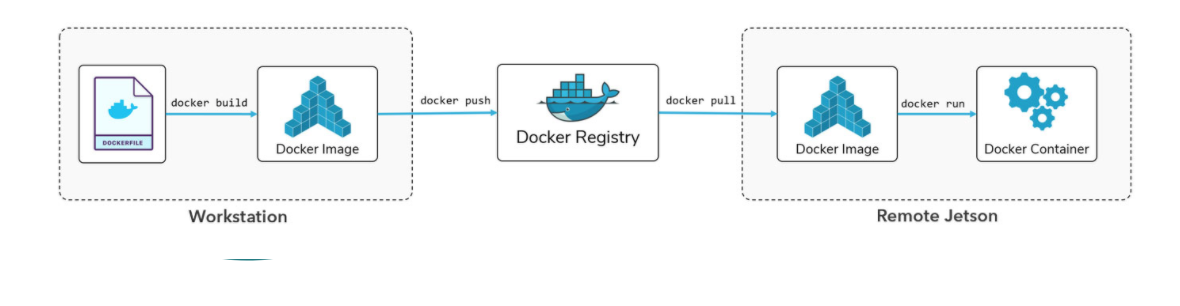
\includegraphics[keepaspectratio=true,scale=0.33]{figuras/deploy-quemu.png}
	\caption{Deploy de uma imagem docker na Jetson \cite{Deploy-Jetson} }
	\label{fig:deploy-jetson}
\end{figure}

Mais informações sobre esse processo podem ser verificados no link a seguir: \href{https://www.stereolabs.com/docs/docker/building-arm-container-on-x86/}{Arm container on x86}.

